%%
%% ****** ljmsamp.tex 13.06.2018 ******
%%
\documentclass[
11pt,%
tightenlines,%
twoside,%
onecolumn,%
nofloats,%
nobibnotes,%
nofootinbib,%
superscriptaddress,%
noshowpacs,%
centertags]%
{revtex4}
\usepackage{ljm}
\usepackage{listings}
\usepackage{amsmath,amsthm,amscd,amsfonts,amssymb}
\usepackage{textcomp}
\usepackage{graphicx}
\usepackage{esvect}
\usepackage{physics}

\lstset{
language=C++,
basewidth=0.5em,
xleftmargin=45pt,
xrightmargin=45pt,
basicstyle=\small\ttfamily,
keywordstyle=\bfseries\underbar,
numbers=left,
numberstyle=\tiny,
stepnumber=1,
numbersep=10pt,
showspaces=false,
showstringspaces=false,
showtabs=false,
frame=trBL,
tabsize=2,
captionpos=t,
breaklines=true,
breakatwhitespace=false,
escapeinside={\%*}{*)}
}

\begin{document}

\titlerunning{Dynamic objects type identification algorithm robustness} % for running heads
\authorrunning{A.~N.~Katulev, A.~N.~Sotnikov, V.~K.~Kemaikin, I.~V.~Kozhukhin} % for running heads
%\authorrunning{First-Author, Second-Author} % for running heads

\title{Robustness of the algorithm of identification of the type of dynamic object found at the finite sequence of 2D background frames of the optoelectron device}

% Splitting into lines is performed by the command \\
% The title is written in accordance with the rules of capitalization.

\author{\firstname{A.~N.}~\surname{Katulev}}
\email[E-mail: ]{katuleva@mail.ru}
\affiliation{Central Research Institute of Aerospace Defense Forces of Ministry of Defense of the Russian Federation, Afanasiy Nikitin Embankment, building 32, Tver, 170026, Russia}

\author{\firstname{A.~N.}~\surname{Sotnikov}}
\email[E-mail: ]{asotnikov@jscc.ru}
\affiliation{Joint Supercomputer Center of the Russian Academy of Sciences - branch of Scientific Research Institute of System Analysis of the Russian Academy of Sciences, Leninsky prospect 32a, Moscow, 119334, Russia}

\author{\firstname{V.~K.}~\surname{Kemaikin}}
\email[E-mail: ]{vk-kem@mail.ru}
\affiliation{State Technical University, Lenin Avenue, building 25, Tver, 170023, Russia}

\author{\firstname{I.~V.}~\surname{Kozhukhin}}
\email[E-mail: ]{kozhukhin@mail.ru}
\affiliation{State Technical University, Lenin Avenue, building 25, Tver, 170023, Russia}

%\noaffiliation % If the author does not specify a place of work.

\firstcollaboration{(Submitted by TODO : SUBMITTER)} % Add if you know submitter.
%\lastcollaboration{ }

\received{TODO : DATE} % The date of receipt to the editor, i.e. December 06, 2017

\begin{abstract}
Here are proposed robustness characteristics of the algorithm of identification of the type of the dynamic object (DO) and the law of probability distribution of identification sufficient statistics, formed by the algorithm under prior uncertainty.
The law is applied for verification and validation of the algorithm.
Wavelet fractal correlation algorithm (WFCA) implements vectorial criterion of ratio of likelihood functions of simple alternative hypotheses - types of DOs, this criterion being invariant to specific features of DO motion trajectories.
The likelihood functions are reconstructed by simulation according to sufficiently representative complexes of implementations of fractal dimensions, energies, wavelet spectra and maximum eigenvalues of biased correlation matrices as functional of the measured coordinates of spatial attitude of various types of real DOs located by the optoelectron device (OED).
The simulation proved  robustness and high efficiency of the algorithm of identification of the type of DOs.
\end{abstract}

%\subclass{TODO : CODE} % Enter 2010 Mathematics Subject Classification.

\keywords{identification algorithm, dynamical object, optoelectronic device} % Include keywords separeted by comma.

\maketitle

% Text of article starts here.

\section{Relevance}

\begin{figure}[h]
\setcaptionmargin{5mm}
\onelinecaptionstrue
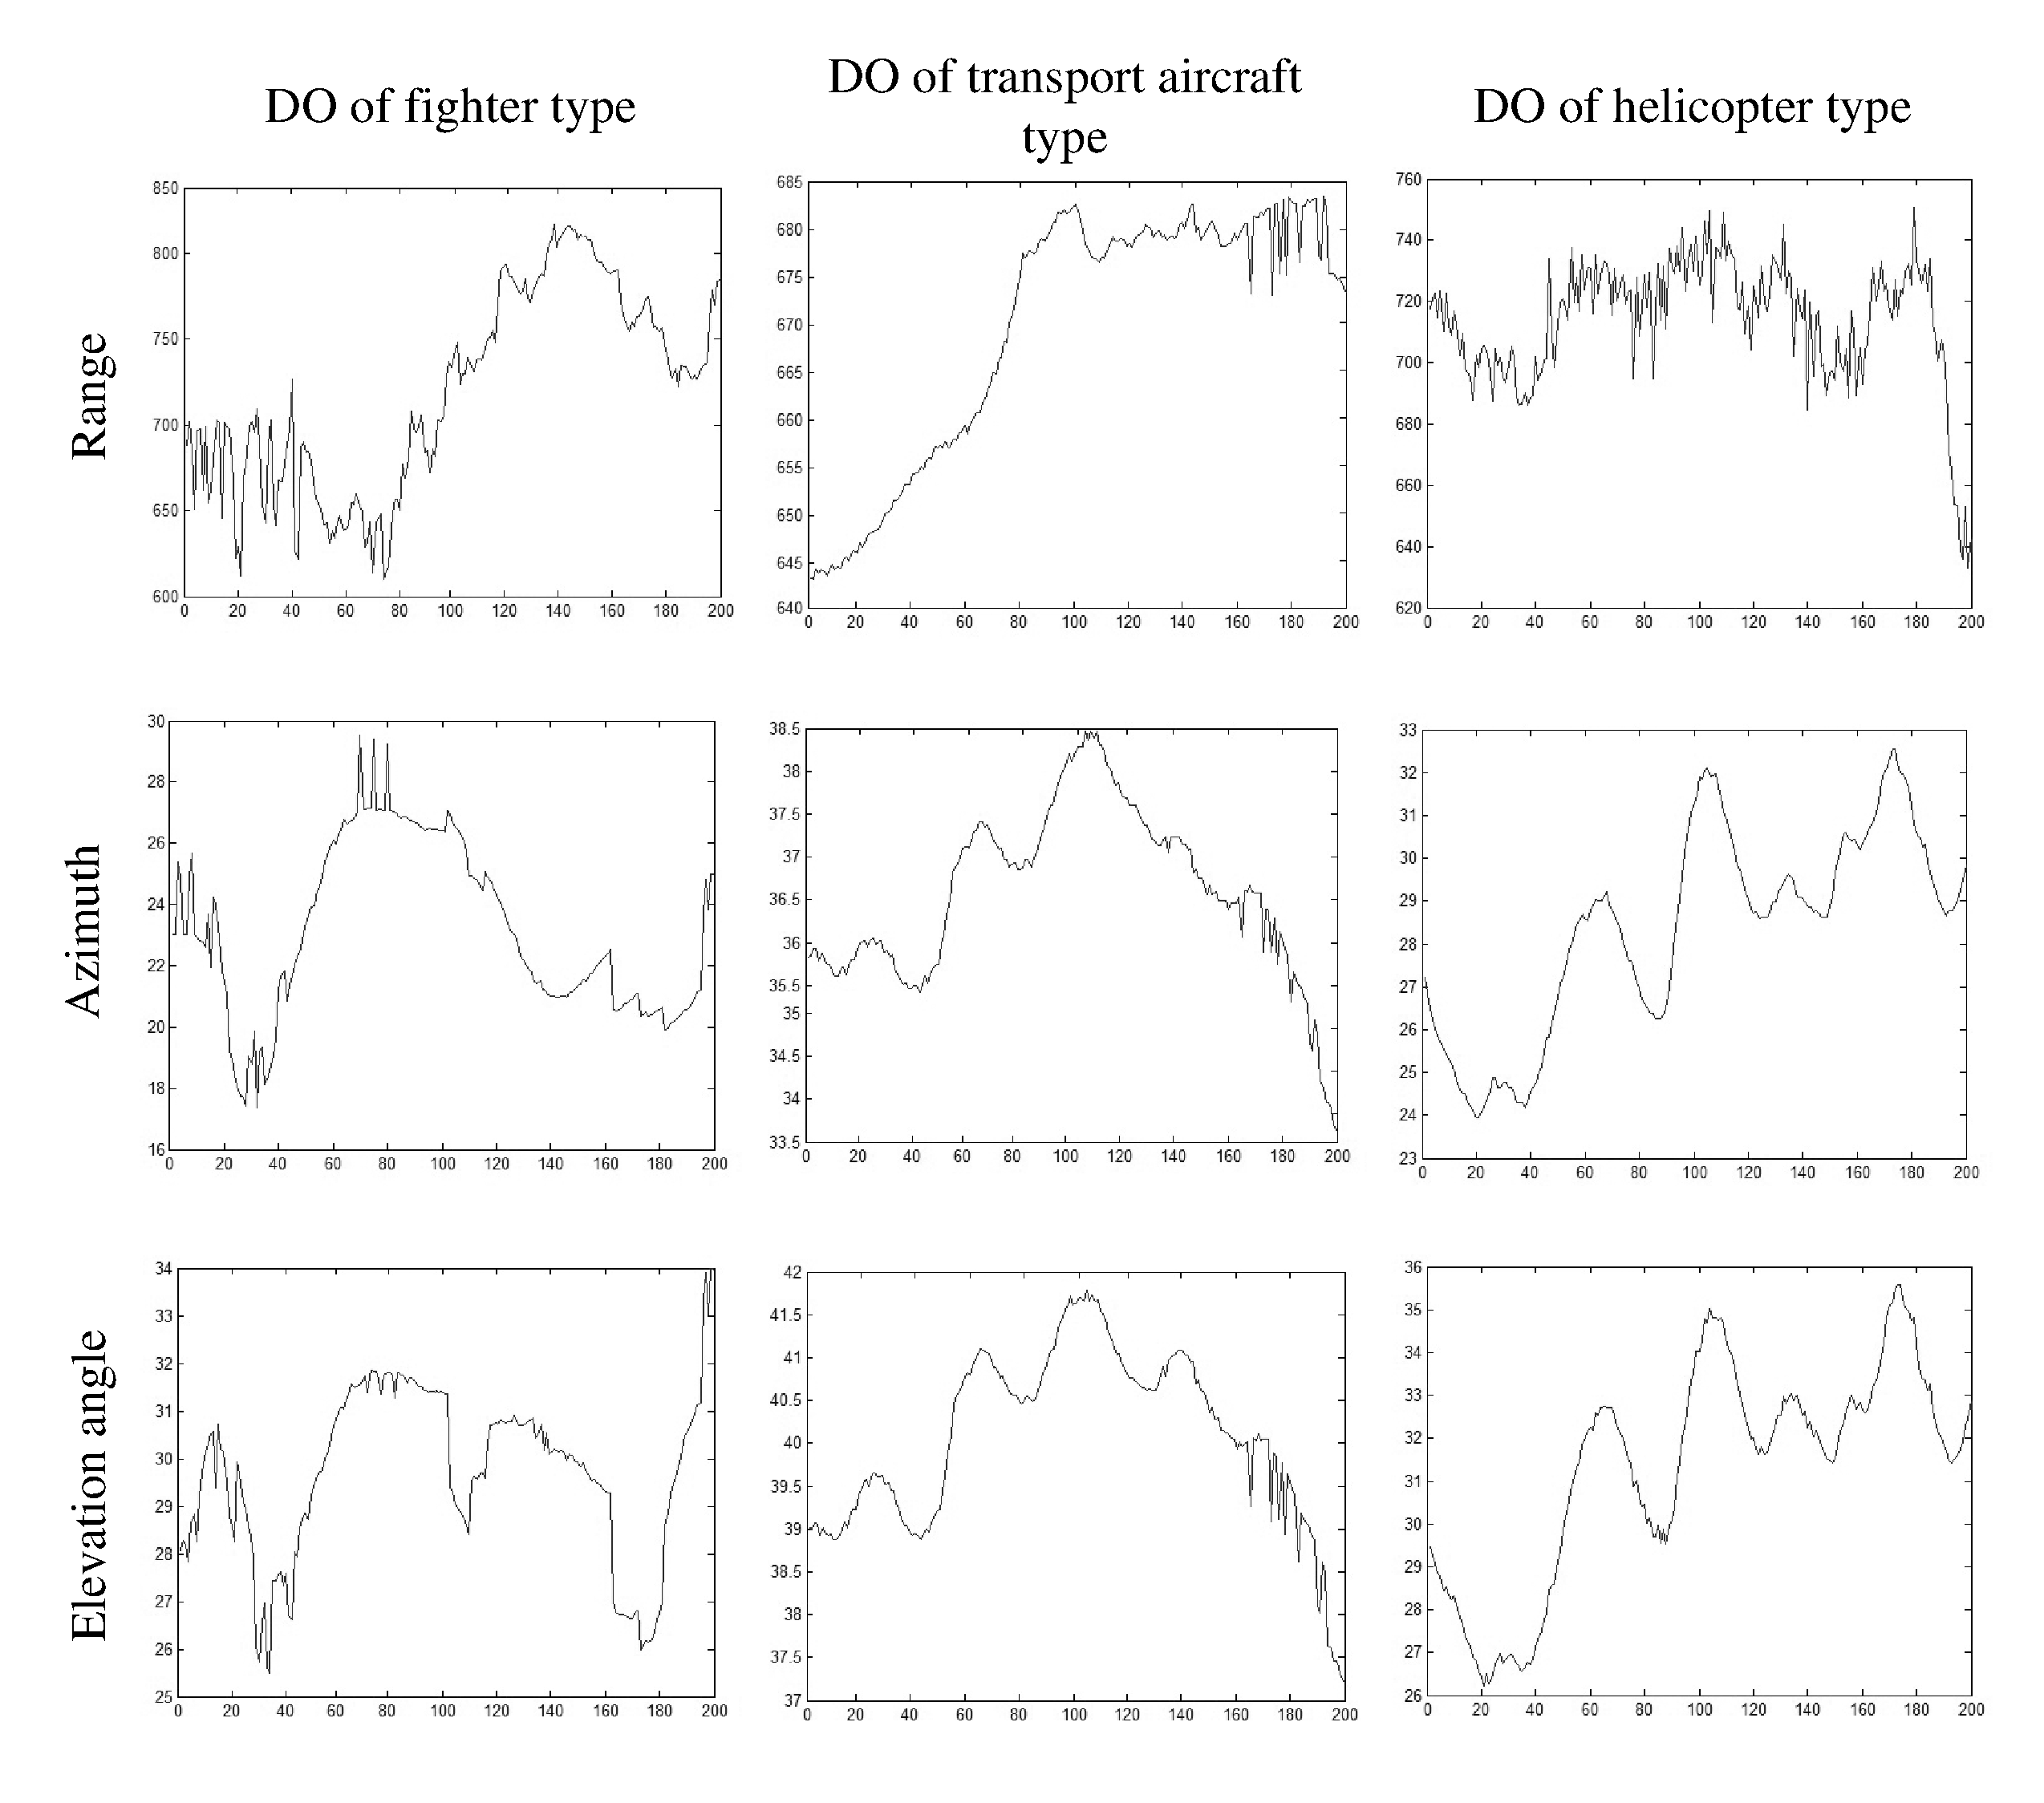
\includegraphics[width=1.0\textwidth]{pics/fig_1_option_1.pdf}
\captionstyle{normal}\caption{The samples of DO coordinate measuring for different angles of standard flight trajectory their observations by OED. Option 1.}\label{fig:fig_1_option_1}
\end{figure}

\begin{figure}[h]
\setcaptionmargin{5mm}
\onelinecaptionstrue
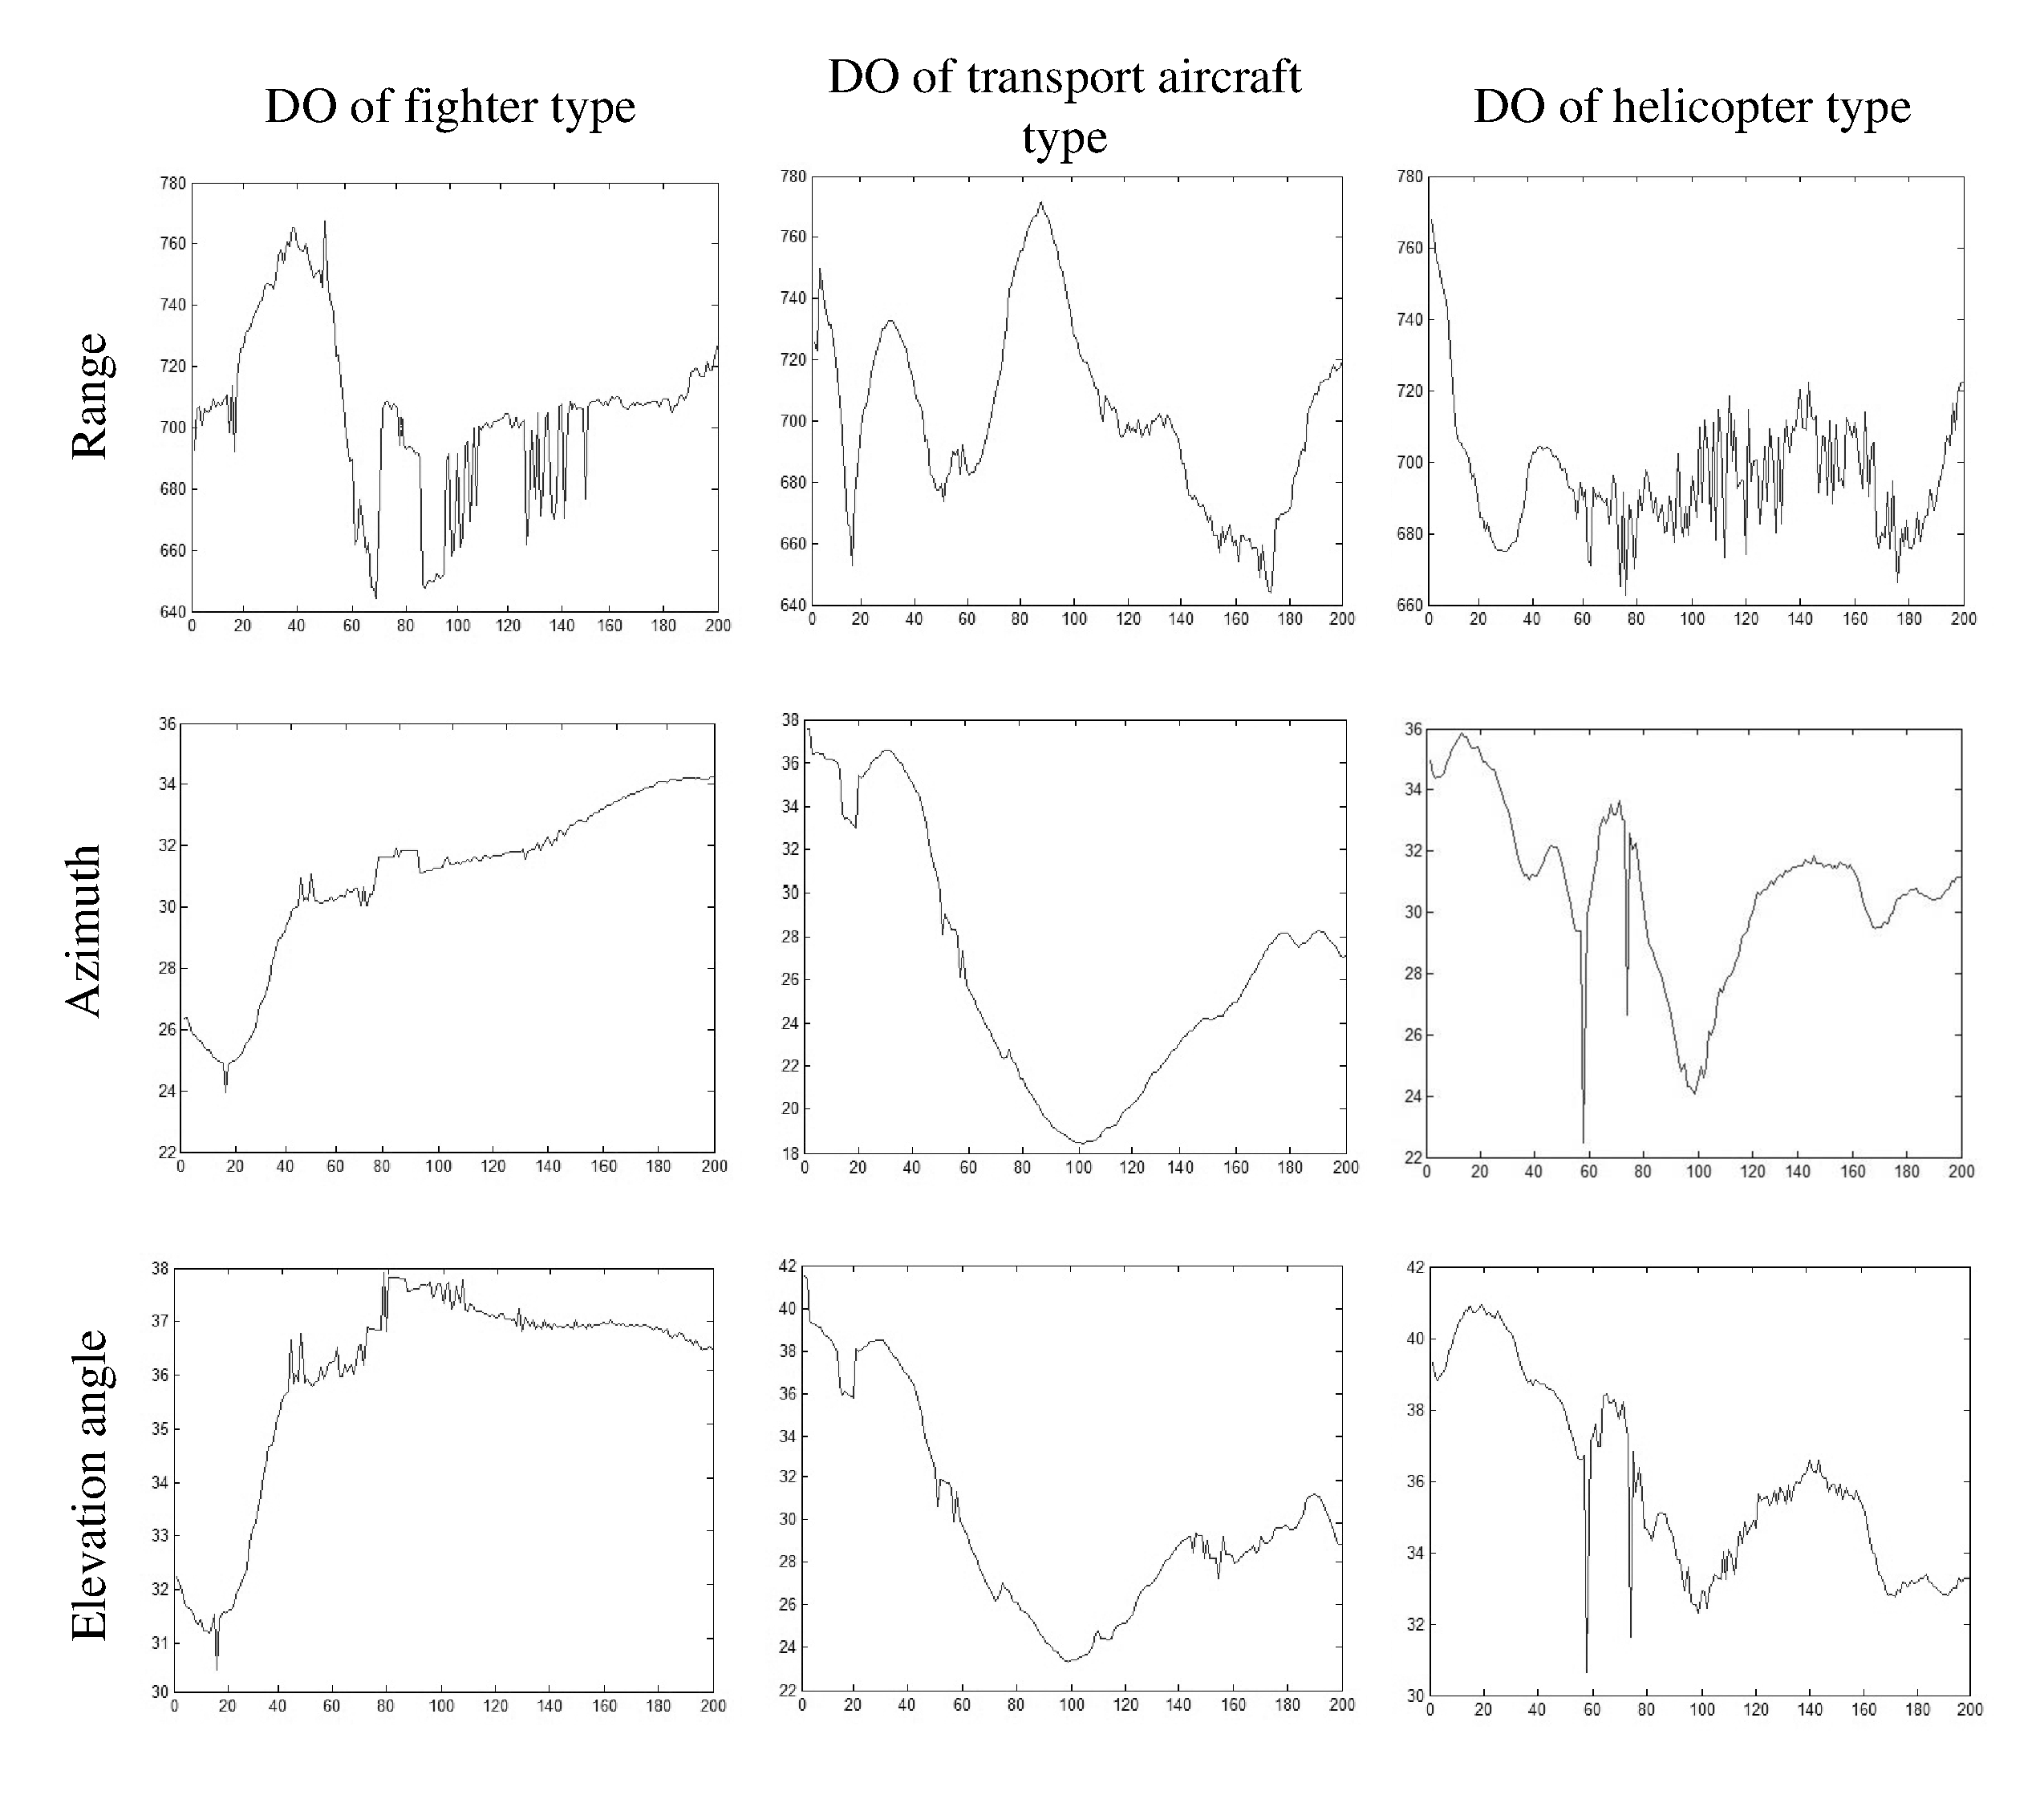
\includegraphics[width=1.0\textwidth]{pics/fig_1_option_2.pdf}
\captionstyle{normal}\caption{The samples of DO coordinate measuring for different angles of standard flight trajectory their observations by OED. Option 2.}\label{fig:fig_1_option_2}
\end{figure}

\begin{figure}[h]
\setcaptionmargin{5mm}
\onelinecaptionstrue
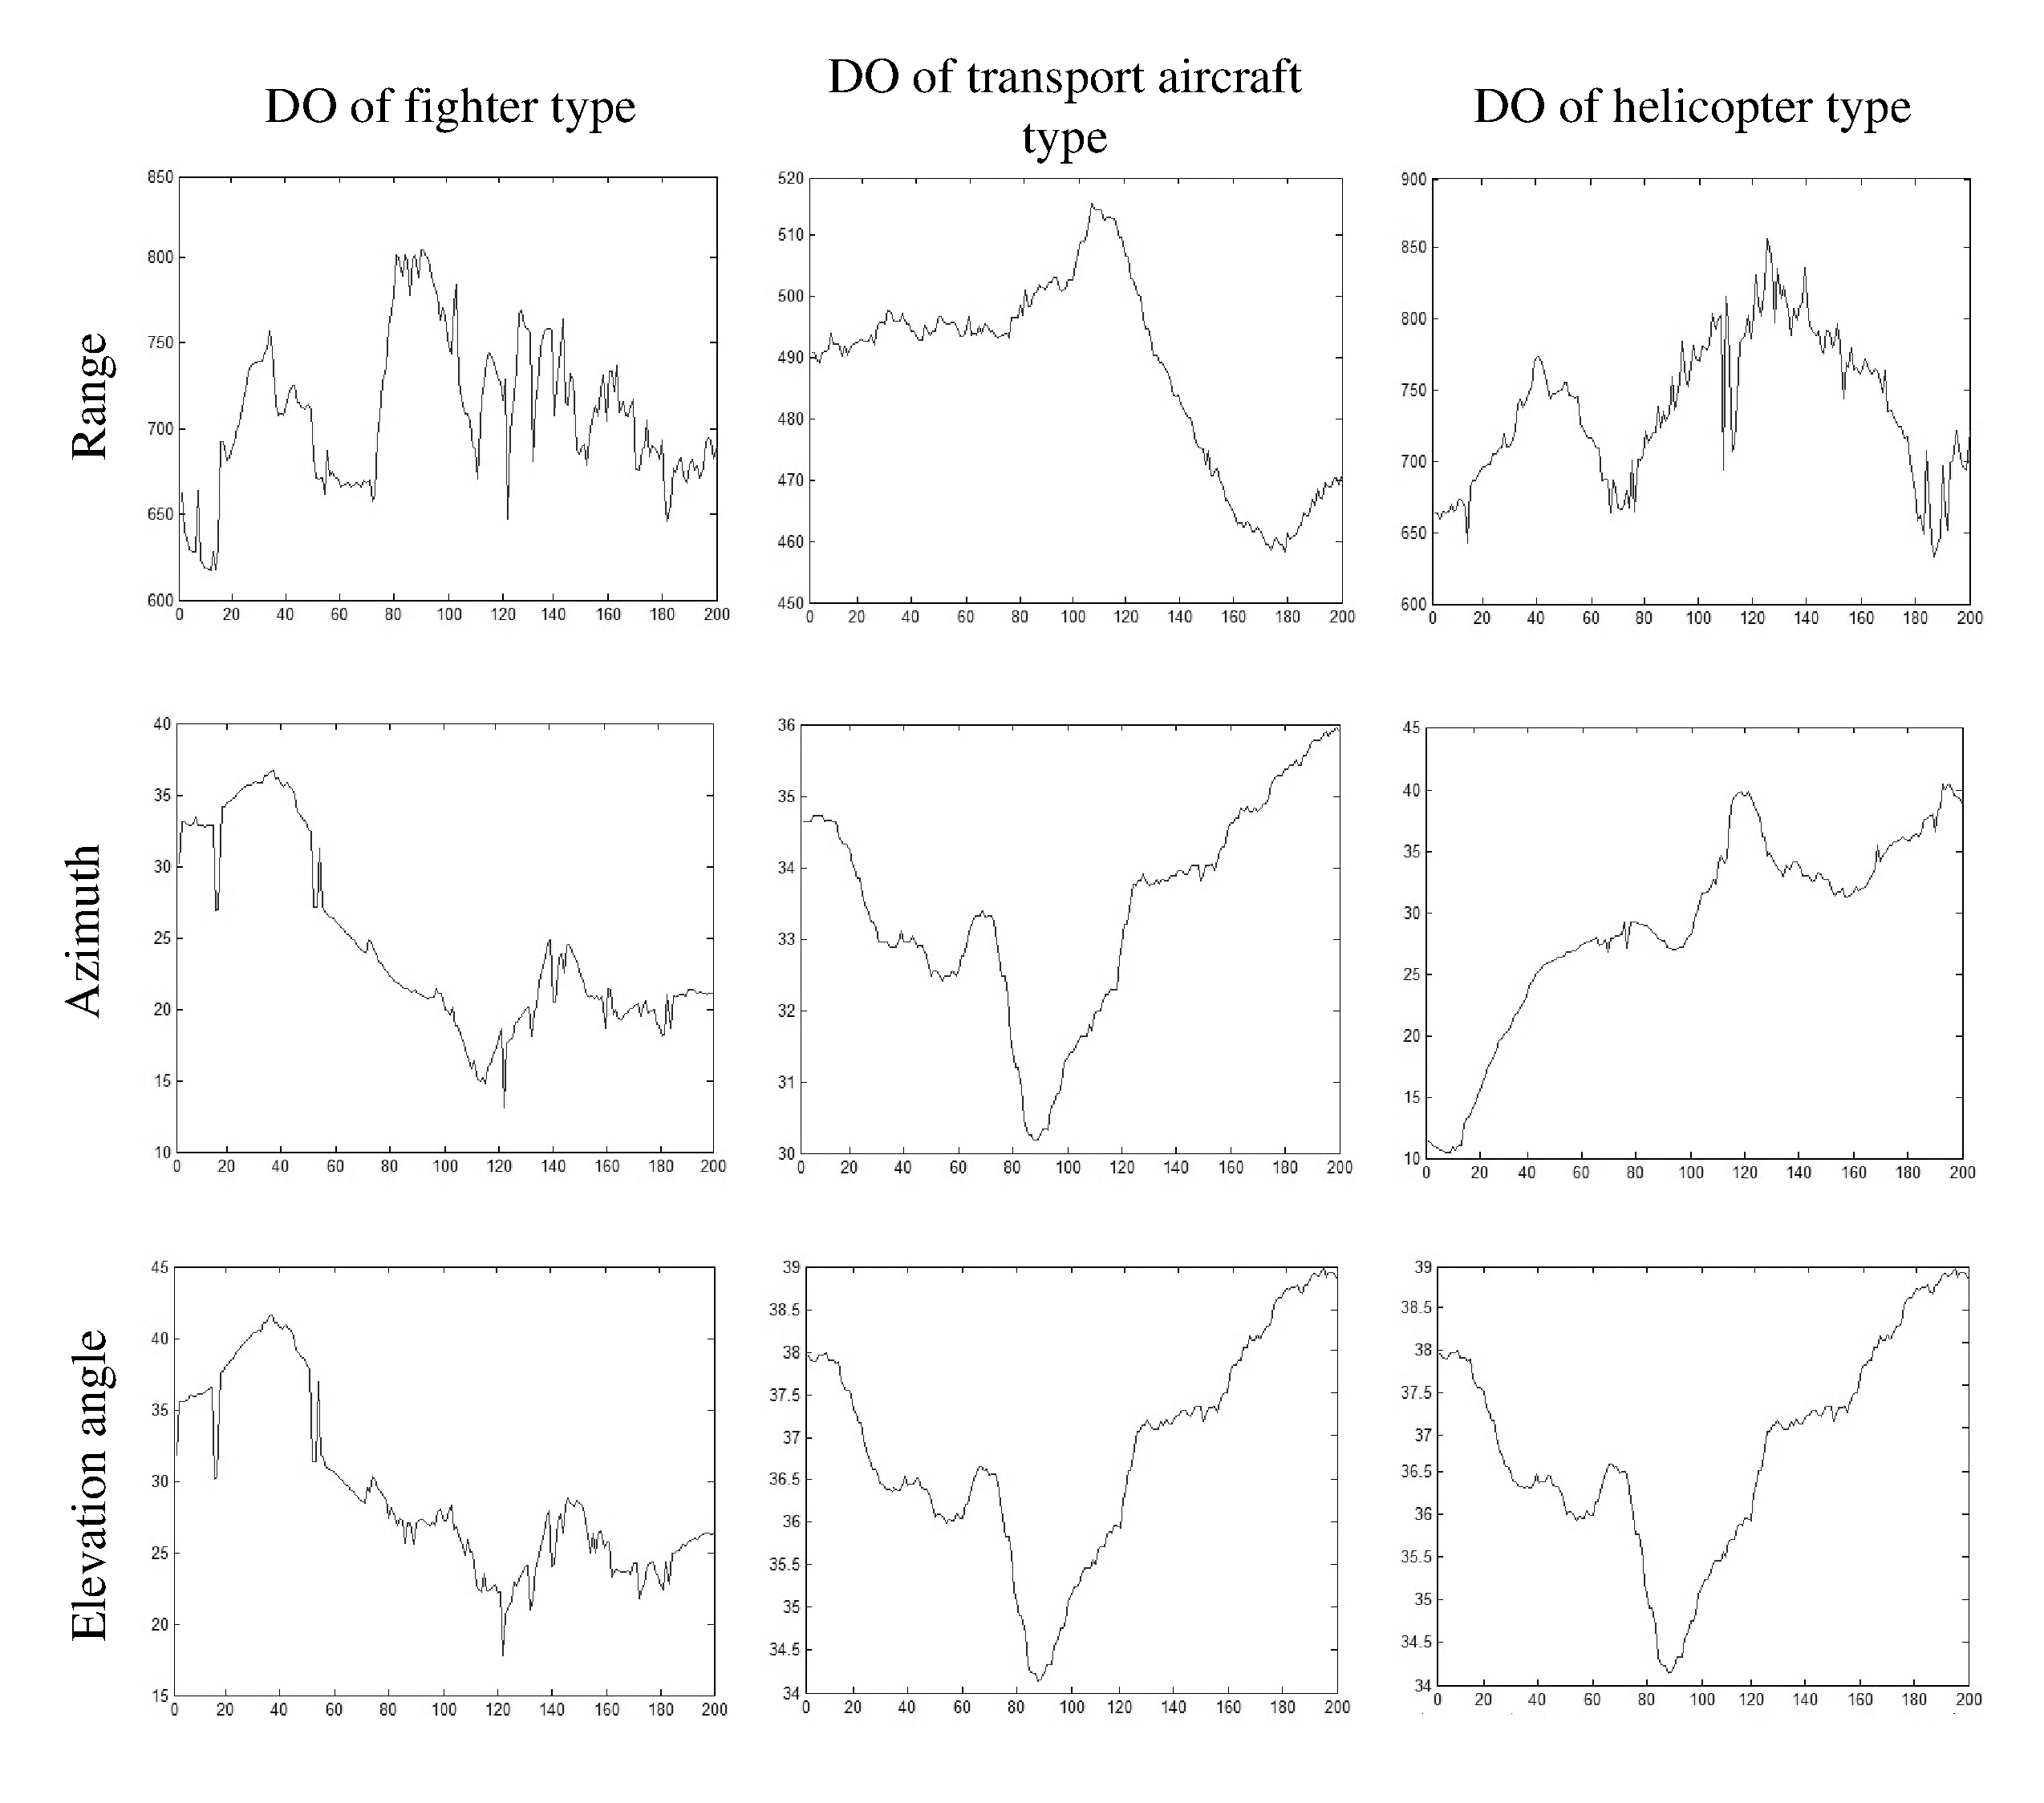
\includegraphics[width=1.0\textwidth]{pics/fig_1_option_3.pdf}
\captionstyle{normal}\caption{The samples of DO coordinate measuring for different angles of standard flight trajectory their observations by OED. Option 3.}\label{fig:fig_1_option_3}
\end{figure}


\section{The objective of article}

objective TODO

\section{Wavelet-fractal-correlation algorithm: the structure and properties}

The structure and computational operations of VFKA are completely determined by expressions of DO type identification criteria based on sufficient statistics: fractal dimensions -- $d(\cdot)$, wavelet spectral energies -- $u(\cdot)$ and maximum eigenvalues -- $\lambda(\cdot)$ for shifted correlation matrices of samples of elevation coordinates measurements for elevation angle -- $\theta$, azimuth -- $\phi$ and elevation angle -- $D$ of DO locating OED (the dot $\cdot$ is a measured coordinate, three types of DO have nine statistics).
 
The sufficiency of each of these statistics is physically determined by the fact that they are calculated directly from samples of DO coordinate measurements as minimal sufficient statistics, and formally it is established by the well-known Rao-Blequella-Kolmogorov theorem: optimal estimates (subject to their existence) are functions of sufficient statistics \cite{bib_07}.
In this case, the validity of the application of the theorem is obvious.
Additionally, we note that in \cite{bib_01}, the authors confirmed the sufficiency property based on the analysis of the likelihood functions of obtaining measurement samples under the condition that they are located in the zone of control of the OED for DO corresponding type which we should recognize (as an option it is considered transport aircraft, fighter and helicopter \cite{bib_08}).
Identification criteria are written as \cite{bib_01} 

\begin{equation}\label{eqn:eqn_1}
\begin{gathered}
\frac{f_d(d(\theta) | p_j, q_j, d(\theta_j), s_j)}{f_d(d(\theta) | p_i, q_i, d(\theta_i), s_i)} \ge 1,
\frac{f_d(d(\phi) | p_j, q_j, d(\phi_j), s_j)}{f_d(d(\phi) | p_i, q_i, d(\phi_i), s_i)} \ge 1,
\frac{f_d(d(D) | p_j, q_j, d(D_j), s_j)}{f_d(d(D) | p_i, q_i, d(D_i), s_i)} \ge 1, \\
\frac{f_u(u(w(\theta)) | p_j, q_j, u(w_j), s_j)}{f_u(u(w(\theta)) | p_i, q_i, u(w_i), s_i)} \ge 1,
\frac{f_u(u(w(\phi)) | p_j, q_j, u(w_j), s_j)}{f_u(u(w(\phi)) | p_i, q_i, u(w_i), s_i)} \ge 1,
\frac{f_u(u(w(D)) | p_j, q_j, u(w_j), s_j)}{f_u(u(w(D)) | p_i, q_i, u(w_i), s_i)} \ge 1, \\
\frac{f_{\lambda}(\lambda(\theta) | p_j, q_j, \lambda(\theta_j), s_j)}{f_{\lambda}(\lambda(\theta) | p_i, q_i, \lambda(\theta_i), s_i)} \ge 1,
\frac{f_{\lambda}(\lambda(\phi) | p_j, q_j, \lambda(\phi_j), s_j)}{f_{\lambda}(\lambda(\phi) | p_i, q_i, \lambda(\phi_i), s_i)} \ge 1,
\frac{f_{\lambda}(\lambda(D) | p_j, q_j, \lambda(D_j), s_j)}{f_{\lambda}(\lambda(D) | p_i, q_i, \lambda(D_i), s_i)} \ge 1,
\end{gathered}
\end{equation}
 
where $f_d(\cdot | \cdot)$, $f_u(\cdot | \cdot)$, $f_{\lambda}(\cdot | \cdot)$ are beta-likelihood functions of samples, provided that they are in the control zone of OED for DO type $s_j$, $j,i = 1,2, \dots, M$, $j \ne i$, $p_j > 0$, $q_i > 0$ -- beta-functions parameters.
 
Criteria (\ref{eqn:eqn_1}) is a vector of independent subtests (independence is determined by the independence of the statistics $d(\theta)$, $d(\phi)$, $d(D)$, $u(w(\theta))$, $u(w(\phi))$, $u(w(D))$, $\lambda(\theta)$, $\lambda(\phi)$, $\lambda(D)$).
 
Directly from (1\ref{eqn:eqn_1} it follows that the structures of the criteria are similar, trans-form after logarithmation to the same type of computational expression and completely determine the sequence of computational operations of the algorithm of DO type identification.

Write this expression, for example, for an algorithm that implements the first criterion from (\ref{eqn:eqn_1}):

\begin{equation}\label{eqn:eqn_2}
\begin{gathered}
(p_j - 1) \ln(u(w(\theta)) - \mu_{j0}) + (q_j - 1) \ln(\mu_{j1} - u(w(\theta))) \\
- (p_i - 1) \ln(u(w(\theta)) - \mu_{i0}) - (q_i - 1) \ln(\mu_{i1} - u(w(\theta))) \ge \\
\ge -\ln{\frac{1}{\mu_{j1} - \mu_{j0}}} - \ln{\frac{\Gamma(p_j + q_j)}{\Gamma(p_j)\Gamma(q_j)}} + (p_j - 1) \ln(\mu_{j1} - \mu_{j0}) + (q_j - 1) \ln(\mu_{j1} - \mu_{j0}) \\
+ \ln{\frac{1}{\mu_{i1} - \mu_{i0}}} + \ln{\frac{\Gamma(p_i + q_i)}{\Gamma(p_i)\Gamma(q_i)}} - (p_i - 1) \ln(\mu_{i1} - \mu_{i0}) + (q_i - 1) \ln(\mu_{i1} - \mu_{i0})
\end{gathered}
\end{equation}

where $\mu_{j0} \le u(w(\theta)) \le \mu_{j1}$, $j,i = 1,2, \dots, M$, $j \ne i$, $\mu_{j0}$, $\mu_{j1}$ are left and right limits of range for values of sample sufficient statistics for identification algorithm.
They are given in \cite{bib_01}.

In this inequality expression, the right-hand side is the threshold level of decision making based on subset DO type identification criterion, and the left side is the recognition statistics as a function of a random variable -- sufficient statistics -- on the wavelet-spectrum energy of a measurements sample for the elevation angle of detecting DO in the current time interval.

From (\ref{eqn:eqn_2}) it can be seen that the recognition statistics is represented by a linear combination of logarithmic functions of sufficient statistics $u(w(\theta))$.
 
Such functions are monotonous, they do not distort the sufficiency of the transformed statistics $u(w(\theta))$ \cite{bib_09,bib_10}.
This means that each component of a linear combination is sufficient statistics as a function of sufficient statistics $u(w(\theta))$ and that a linear combination as a whole as statistics of DO type identification for a particular criterion is sufficient statistics, naturally, random, since the sample is finite.
At the same time, we also note that the sufficiency of statistics is a consequence of the sufficiency properties of each initially considered likelihood ratio \cite{bib_09} and that with a sufficiently large sample, the likelihood ratio statistics are consistent and robust \cite{bib_10}.

The established properties of the statistics of the left-hand side of (\ref{eqn:eqn_2}) are sufficient conditions for assessing the stability of a particular DO type identification algorithm.

The necessary conditions are the stability of each initial sufficient statistics for the algorithm: fractal dimension -- $d(\cdot)$ , energy of the wavelet spectrum -- $u(\cdot)$, maximum eigenvalue -- $\lambda(\cdot)$ as a function of a sample of OED measurements of position for identifying DO, otherwise, as functions of minimal sufficient statistics obtained from the DO detection time interval. 

The stability of private algorithms and the initial sufficient statistics for them together determine the stability property of DO type identification algorithm that implements a vector of criteria (\ref{eqn:eqn_1}).


\section{The stability of the initial sufficient statistics for the DO type identification algorithm}

Taking into account that the initial data: the fractal dimension, the energy of the wavelet spectrum and the maximum eigenvalue generated for the DO type identification algorithm are sufficient statistics, here we will show that they and the algorithms for their formation are stable.

To that end, in the statistical approach, we use the law of large numbers and the central limit theorem as a theoretical basis \cite{bib_11} for determining stability and algorithms for estimating sufficient statistics for DO type identification algorithm, and the statistics itself.
The validity of the approach comes from the fact that

-- OED measurement sample for each coordinate of the DO detected position is a set of realizations of a sufficiently large volume of independent equally distributed random variables according to the same law, a priori unknown;

-- sufficient statistics for each particular algorithm of DO type identification are estimates of the expectation for the fractal dimension, the energy of the wavelet spectrum and the maximum eigenvalue.
They are determined by empirical variances.
The evaluation of the third and fourth moments are not affected, since they are completely and unambiguously determined by empirical estimates of the expectation and variance for the beta distribution.

Now, to determine the stability index of the first two moments for sufficient statistics, we use the fundamental theory of confidence estimation of the expectation and variance, which asserts a unique functional relationship among the sample size, the number of observations, the accuracy of the estimated parameter as a measure of the minimum length of the confidence interval of the parameter estimate and the acceptable (required) confidence level proximity parameter estimates to the true (unknown) value.

The measure of localization of the estimated parameter by the confidence interval at a given confidence level and the final sample size is an indicator of the stability of the assessment.

In the problem of estimating the first moment -- the mathematical expectation with unknown true variance $l$ -- the measure of localization of the estimate by the confidence interval, the confidence probability -- $\beta$, the estimate of the standard deviation $s$ and the sample size -- $n$ are related by the expression $l = 2sC_{\beta}/\sqrt{n}$, where $C_{\beta}$ is the required (admissible given) confidence probability $\beta$ from the condition: Laplace function $\Phi_n(C_{\beta}) = \beta$ with a sufficiently large sample $n$ \cite{bib_13,bib_14}.

In the problem of estimating the second moment -- the standard deviation with an unknown expectation, $l_{\sigma} = |s - \sigma|$ -- the localization measure -- $s$ the standard deviation, the sample size -- $n$ and the confidence level -- $\beta$ are related $l_{\sigma} = st_{\beta}/\sqrt{n}$, where $t_{\beta}$ is the value $\beta$ of the condition that (for large $n$) the Laplace function $\Phi_n(t_{\beta})$.

So, in the case $C_{\beta} = 1.6$, defined in \cite{bib_01} by the "no-overrunning" condition of selective sufficient statistics beyond the unit interval and corresponding to a confidence level of $0.89$ when approximating the probability distribution law of the deviation of the expectation estimate from the true value by a normal law \cite{bib_13}, the localization measure $l = 2sC_{\beta}/\sqrt{n} = 2 \cdot 0.36 \cdot 1.6 / 10 = 0.1192$ for $n = 100$ and estimate of standard deviation $s = 0.36$.
 
It can be seen that in this case there is a very good approximation of the value of the estimated parameter -- the mathematical expectation to the true one, and the estimate can be considered consistent, that is, stable.
The algorithm for generating an estimate as sufficient statistics is also stable.
Similar holds for estimating standard deviation.

Additionally, under conditions of a priori uncertainty, the adoption of a normal approximation of an unknown law is also based on the well-known \cite{bib_16} property of a normal law: the entropy of a random variable has the largest value with the same standard deviation if the probability distribution of a random variable is normal.

Thus, sufficient statistics: the estimates of the first two moments of the fractal dimension, the energy of the wavelet spectrum, and the maximum eigenvalue, which are generated for particular DO type indefication algorithms, and the algorithms for cal-culating them are stable.
At the same time, $l$ and $l_{\sigma}$ are measures of localization of estimates in the vicinity of their true values were found as the least favorable -- guaranteed for an acceptable level of confidence probability: without performing the operation of minimizing the interval.

If we now take into account \cite{bib_01} that the mentioned sufficient statistics take only positive values and only from finite intervals of their values, then the following becomes true: the initial sufficient statistics for (\ref{eqn:eqn_1} are subject to probability distributions from the class of beta distributions.
The latter, as is known \cite{bib_12}, are uniquely determined by only two parameters $p_j > 0$, $q_j > 0$ -- the DO type index.
These parameters, as noted, in turn, are uniquely determined by estimates of mathematical expectations -- $m_{j}^{*}$ and variances -- $s^2 = {\sigma_{j}^{*}}^2$ sufficient statistics (in this case, guaranteed estimates): the parameters are one-to-one associated with these estimates by rational functions of the form $p_j = (m_{j}^{*} - {\sigma_{j}^{*}}^2) / [({\sigma_{j}^{*}}^2 / m_{j}^{*}) - m_{j}^{*}]$ and $q_j = (p_j / m_{j}^{*}) - p_j$.

With such communication functions, the parameters, $p_j$, $q_j$, by virtue of the stability $m_{j}^{*}$ and ${\sigma_{j}^{*}}^2$ and assurance of their values, are stable \cite{bib_16}.
From this it follows that in this sense, the beta laws of the probability distribution of sufficient statistics of the fractal dimension, the energy of the wavelet spectrum, and the maximum eigenvalue are stable as laws that are completely determined by their stable parameters $p_j > 0$, $q_j > 0$.
The laws are represented by power functions from sufficient statistics and are determined from samples of a sufficiently large amount of measurements of the coordinates of the position of the de-tected DO by OED with different features of the flight trajectory, sighting DO and background conditions (Fig.~\ref{fig:fig_1_option_1}, Fig.~\ref{fig:fig_1_option_2}, Fig.~\ref{fig:fig_1_option_3}).


\section{The stability of the recognition algorithm type}

stability 2 TODO

\section{The probability distribution law of statistics recognition of DO type. Stability properties.}

\textit{Definition:} DO type identification statistics is a random variable of the type of the left part of the rule (2).

To evaluate the efficiency of the algorithm, it is naturally necessary to know the law of probability distribution of the recognition statistics, the threshold level for deciding on the type of the detected DO and the stability properties of the law.

Obviously, from the structure of the left-hand side of (2), the law can be established subject to the known laws of the distribution of the probabilities of each of its terms as sufficient statistics. The laws of the terms are conditional: they are established provided that DO are located in the OED control zone for each alternative type.

The terms are the functions of samples of independent measurements of the coordinates of the elevation angle of either the azimuth or the distance in the time interval for detecting the DO by OED.

Under such circumstances, a formal solution to the problem of restoring the desired law of statistics of the form of the left part (2) as a linear combination is reduced to performing the sequence of the following operations for the measurement samples and the functions of them:

Under such circumstances, a formal solution to the problem of restoring the desired law of statistics of the form of the left part (2) as a linear combination is reduced to performing the sequence of the following operations for the measurement samples and the functions of them:

1. Conversion of samples to the form of primary sufficient statistics: fractal dimensions $d(\theta)$, $d(\varphi)$, $d(D)$, wavelet spectral energy  $ u(w(\theta)) $, $ u(w(\varphi)) $, $ u(w(D)) $ and maximum eigenvalues $ \lambda(\theta) $, $ \lambda(\varphi) $, $ \lambda(D) $  . The transformation is carried out by algorithmically realized linear functionals and operators, their substantive essence is disclosed in the previous subsection.

2. Calculation of the laws of probability distribution of sufficient statistics $d(\theta)$, $d(\varphi)$, $d(D)$, $ u(w(\theta)) $, $ u(w(\varphi)) $,  $ \lambda(\theta) $, $ \lambda(\varphi) $, $ \lambda(D) $.

The type of laws for various conditions - the types of DO, observed by the ODE, is set by modeling, their mathematical description is presented in [1]. These are beta distributions with appropriate parameters for alternative DO types.

3. Calculation of probability distribution laws for function statistics

\begin{equation*}
({{p}_{j}}-1)\ln (d(\theta )-{{\mu }_{j0}}),\ ...\ ({{q}_{j}}-1)\ln ({{\mu }_{j1}}-d(\theta )),
\end{equation*}

\begin{equation*}
({{p}_{j}}-1)\ln (d(\varphi )-{{\mu }_{j0}}),\ ...\ ({{q}_{j}}-1)\ln ({{\mu }_{j1}}-d(\varphi )),
\end{equation*}

\begin{equation*}
({{p}_{j}}-1)\ln (d(D)-{{\mu }_{j0}}),\ ...\ ({{q}_{j}}-1)\ln ({{\mu }_{j1}}-d(D)),
\end{equation*}

\begin{equation*}
({{p}_{j}}-1)\ln (u(w(\theta ))-{{\mu }_{j0}}),\ ...\ ({{q}_{j}}-1)\ln ({{\mu }_{j1}}-u(w(\theta ))),
\end{equation*}

\begin{equation*}
({{p}_{j}}-1)\ln (u(w(\varphi ))-{{\mu }_{j0}}),\ ...\ ({{q}_{j}}-1)\ln ({{\mu }_{j1}}-u(w(\varphi ))),
\end{equation*}

\begin{equation*}
({{p}_{j}}-1)\ln (u(w(D))-{{\mu }_{j0}}),\ ...\ ({{q}_{j}}-1)\ln ({{\mu }_{j1}}-u(w(D))),
\end{equation*}

\begin{equation*}
({{p}_{j}}-1)\ln (\lambda (\theta ))-{{\mu }_{j0}}),\ ...\ ({{q}_{j}}-1)\ln ({{\mu }_{j1}}-\lambda (\theta )),
\end{equation*}

\begin{equation*}
({{p}_{j}}-1)\ln (\lambda (\varphi ))-{{\mu }_{j0}}),\ ...\ ({{q}_{j}}-1)\ln ({{\mu }_{j1}}-\lambda (\varphi )),
\end{equation*}

\begin{equation*}
({{p}_{j}}-1)\ln (\lambda (D))-{{\mu }_{j0}}),\ ...\ ({{q}_{j}}-1)\ln ({{\mu }_{j1}}-\lambda (D)).
\end{equation*}

The laws are calculated using the well-known formula $ \psi (y)=f(\phi (y))\left| {\phi }'(y) \right| $, where $ y=\xi (x) $, $ \xi $ is a differentiable monotonic function, $ \varphi $ is an inverse function with respect to a function  $ \xi $, is a density of a random variable $ y $, $f(x|{{s}_{j}})$ a density of a random variable  subject to the condition $ {{s}_{j}} $ of the DO type.

In the case, for the component, $({{p}_{j}}-1)\ln [u(w(\theta ))-{{\mu }_{j0}}]$ taking into account the notation in the formula for $\psi (y)$ have $y=({{p}_{j}}-1)\ln (u(w(\theta ))-{{\mu }_{j0}})$ or this $x=u(w(\theta ))=\exp \{y/({{p}_{j}}-1)\}+{{\mu }_{j0}}=\phi (y)$ is  a random variable with a beta-distribution density ($\theta $ - designation of the non-random elevation position) and the probability distribution density of a random variable has the form.


\begin{equation*}
\begin{gathered}
\psi (y|{{s}_{j}})=f(\phi (y|{{s}_{j}})\left| {\phi }'(y) \right|=f(\exp \{y/({{p}_{j}}-1)\}+{{\mu }_{i0}})\left| (1/({{p}_{j}}-1))\exp \{y/({{p}_{j}}-1)\} \right|= \\ 
  =\frac{\left| (1/({{p}_{j}}-1)) \right|\exp \{y/({{p}_{j}}-1)\}}{({{\mu }_{j1}}-{{\mu }_{j0}})}\frac{\Gamma ({{p}_{j}}+{{q}_{j}})}{\Gamma ({{p}_{j}})\Gamma ({{q}_{j}})} \times \\
\times {{\left( \frac{\exp \{y/({{p}_{j}}-1)\}+{{\mu }_{i0}}}{{{\mu }_{j1}}-{{\mu }_{j0}}} \right)}^{{{p}_{j}}-1}}{{\left( 1-\frac{\exp \{y/({{p}_{j}}-1)\}+{{\mu }_{j0}}}{{{\mu }_{j1}}-{{\mu }_{j0}}} \right)}^{{{q}_{j}}-1}} \\ 
\end{gathered}
\end{equation*}


Below we will consider the option $u(w(\theta ))\in [{{\mu }_{j0}}=0,{{\mu }_{j1}}=1]$. The density $\psi (y|{{s}_{j}})$ will be determined only on the negative semi-axis of the values, that is, on the interval - $\infty \le \ y=\left| {{p}_{j}}-1 \right|\ln (u(w(\theta )))\le \ 0$,

\begin{equation*}
\begin{gathered}
\psi (\left. y \right|{{s}_{j}})=(1/\left| {{p}_{j}}-1 \right|)\exp \{y/\left| {{p}_{j}}-1 \right|\}\frac{\Gamma ({{p}_{j}}+{{q}_{j}})}{\Gamma ({{p}_{j}})\Gamma ({{q}_{j}})}{{\left( \exp \{y/\left| {{p}_{j}}-1 \right|\} \right)}^{{{p}_{j}}-1}}{{\left( 1-\exp \{y/\left| {{p}_{j}}-1 \right|\} \right)}^{{{q}_{j}}-1}}
\end{gathered}
\end{equation*}

and we can see all other random variables type $\left| {{p}_{i}}-1 \right|\ln u(w(\theta ))$ will have the same type of density, derived from (1).

Acting in a similar way, we obtain the conditional probability density distribution of random variables of the type $\nu =\left| {{q}_{j}}-1 \right|\ln [1-u(w(\theta ))]$; density is written as

\begin{equation*}
\begin{gathered}
\psi (\left. \nu  \right|{{s}_{j}})=f(\phi (\left. \nu  \right|{{s}_{j}})\left| \phi '(\nu ) \right|=f(1-\exp \left\{ {\nu }/{\left| {{q}_{j}}-1 \right|}\; \right\})\left| ({1}/{\left| {{q}_{j}}-1 \right|)\exp \left\{ {\nu }/{\left| {{q}_{j}}-1 \right|}\; \right\}}\; \right|
\end{gathered}
\end{equation*}

and given that $f({{\mu }_{j1}}-\exp \{\nu /({{q}_{j}}-1)\}$ is a beta distribution, in the form

\begin{equation*}
\begin{gathered}
\psi (\left. \nu  \right|{{s}_{j}})=(1/\left| {{q}_{j}}-1 \right|)\exp \{\nu /\left| {{q}_{j}}-1 \right|\}\frac{\Gamma ({{p}_{j}}+{{q}_{j}})}{\Gamma ({{p}_{j}})\Gamma ({{q}_{j}})} \times \\
\times {{\left( 1-\exp \{\nu /\left| {{q}_{j}}-1 \right|\} \right)}^{{{p}_{j}}-1}}{{\left( \exp \{\nu /\left| {{q}_{j}}-1 \right|\} \right)}^{{{q}_{j}}-1}}.
\end{gathered}
\end{equation*}

and note that the laws obtained $\psi (y|{{s}_{j}})$ and $\psi (\nu |{{s}_{j}})$ do not preserve the form of the beta law: they describe random variables $y$ and$\nu $, taking values from an interval $(-\infty ,0)$.

4. Calculation of probability distribution laws for statistics of functions of the form

\begin{equation*}
({{p}_{j}}-1)\ln (d(\theta )-{{\mu }_{j0}})-({{p}_{i}}-1)\ln (d(\theta )-{{\mu }_{i0}}),\ ...\ ({{q}_{j}}-1)\ln ({{\mu }_{j1}}-d(\theta ))-({{q}_{i}}-1)\ln ({{\mu }_{i1}}-d(\theta ))
\end{equation*}

\begin{equation*}
({{p}_{j}}-1)\ln (d(\varphi )-{{\mu }_{j0}})-({{p}_{i}}-1)\ln (d(\varphi )-{{\mu }_{i0}}),\ ...\ ({{q}_{j}}-1)\ln ({{\mu }_{j1}}-d(\varphi ))-({{q}_{i}}-1)\ln ({{\mu }_{i1}}-d(\varphi ))
\end{equation*}

\begin{equation*}
({{p}_{j}}-1)\ln (d(D)-{{\mu }_{j0}})-({{p}_{i}}-1)\ln (d(D)-{{\mu }_{i0}}),\ ...\ ({{q}_{j}}-1)\ln ({{\mu }_{j1}}-d(D))-({{q}_{i}}-1)\ln ({{\mu }_{i1}}-d(D))
\end{equation*}

\begin{equation*}
\begin{gathered}
({{p}_{j}}-1)\ln (u(w(\theta ))-{{\mu }_{j0}})-({{p}_{i}}-1)\ln (u(w(\theta ))-{{\mu }_{i0}}),\ ...\ ({{q}_{j}}-1)\ln ({{\mu }_{j1}}-u(w(\theta )))- \\
- ({{q}_{i}}-1)\ln ({{\mu }_{i1}}-u(w(\theta )))
\end{gathered}
\end{equation*}

\begin{equation*}
\begin{gathered}
({{p}_{j}}-1)\ln (u(w(\varphi ))-{{\mu }_{j0}})-({{p}_{i}}-1)\ln (u(w(\varphi ))-{{\mu }_{i0}}),\ ...\ ({{q}_{j}}-1)\ln ({{\mu }_{j1}}-u(w(\varphi )))- \\
- ({{q}_{i}}-1)\ln ({{\mu }_{i1}}-u(w(\varphi )))
\end{gathered}
\end{equation*}

\begin{equation*}
\begin{gathered}
({{p}_{j}}-1)\ln (u(w(D))-{{\mu }_{j0}})-({{p}_{i}}-1)\ln (u(w(D))-{{\mu }_{i0}}),\ ...\ ({{q}_{j}}-1)\ln ({{\mu }_{j1}}-u(w(D)))- \\
- ({{q}_{i}}-1)\ln ({{\mu }_{i1}}-u(w(D)))
\end{gathered}
\end{equation*}

\begin{equation*}
({{p}_{j}}-1)\ln (\lambda (\theta )-{{\mu }_{j0}})-({{p}_{i}}-1)\ln (\lambda (\theta )-{{\mu }_{i0}}),\ ...\ ({{q}_{j}}-1)\ln ({{\mu }_{j1}}-\lambda (\theta ))-({{q}_{i}}-1)\ln ({{\mu }_{i1}}-\lambda (\theta ))
\end{equation*}

\begin{equation*}
({{p}_{j}}-1)\ln (\lambda (\varphi )-{{\mu }_{j0}})-({{p}_{i}}-1)\ln (\lambda (\varphi )-{{\mu }_{i0}}),\ ...\ ({{q}_{j}}-1)\ln ({{\mu }_{j1}}-\lambda (\varphi ))-({{q}_{i}}-1)\ln ({{\mu }_{i1}}-\lambda (\varphi ))
\end{equation*}

\begin{equation*}
({{p}_{j}}-1)\ln (\lambda (D)-{{\mu }_{j0}})-({{p}_{i}}-1)\ln (\lambda (D)-{{\mu }_{i0}}),\ ...\ ({{q}_{j}}-1)\ln ({{\mu }_{j1}}-\lambda (D))-({{q}_{i}}-1)\ln ({{\mu }_{i1}}-\lambda (D))
\end{equation*}

and establishing the properties of the distribution laws of these statistics for ${{\mu }_{j0}}=0,\text{ }{{\mu }_{j1}}=1$.

It can be seen that the probability densities of differences of equally distributed random variables should be calculated, compared with (1) for the alternative DO types of  ${{s}_{j}}$ and ${{s}_{i}}$. To do this, we use the formula of the composition of the laws of the distribution of independent random variables. $\left| {{p}_{j}}-1 \right|\ln u(w(\theta ))$ и $\left| {{p}_{i}}-1 \right|\ln u(w(\theta ))$.

The desired density is

\begin{equation*}
{{g}_{y-\nu }}({{z}_{1}}|{{s}_{j}},{{s}_{i}})=\int\limits_{\min \{y\}}^{\max \{y\}}{{{\psi }_{Y}}(y|{{s}_{j}}){{\psi }_{\nu }}((y-{{z}_{1}})|{{s}_{i}})dy}
\end{equation*}

where ${{z}_{1}}=y-\nu =\left| {{p}_{j}}-1 \right|\ln u(w(\theta ))-\left| {{p}_{i}}-1 \right|\ln u(w(\theta ))$ and for ${{\mu }_{j0}}=0,\ {{\mu }_{j1}}=1$ and ${{\mu }_{i0}}=0,\ {{\mu }_{i1}}=1\quad u(w(\theta )\in \left[ 0,1 \right]$, density of sufficient statistics $y$ and $\nu $ for DO types $j,i=1,2,\ ...\ ,M,\ j\ne i$, are not equal to zero in the intervals $-\infty \le \left| {{p}_{j}}-1 \right|\ln u(w(\theta ))\le 0$, $-\infty \le \left| {{p}_{i}}-1 \right|\ln u(w(\theta ))\le 0$ for each $j$, $i$. In this case, the density ${{\psi }_{y}}(y|{{s}_{j}})$ is nonzero at $-\infty \le y\le 0$, and the density ${{\psi }_{\nu }}((y-{{z}_{1}})|{{s}_{i}})$ is nonzero at $y-{{z}_{1}}\le 0$ or $y\le {{z}_{1}}$, $-\infty \le {{z}_{1}}\le \infty $, the statistics is unlimited and the required density is written in such convolutions:

as ${{z}_{1}}\le 0$ ${{g}_{y-\nu }}({{z}_{1}}|{{s}_{j}},{{s}_{i}})=\int\limits_{-{{\infty }_{1}}}^{-{{z}_{1}}}{{{\psi }_{Y}}(y|{{s}_{j}}){{\psi }_{\nu }}((y-{{z}_{1}})|{{s}_{i}})dy},$

and as ${{z}_{1}}>0$ ${{g}_{y-\nu }}({{z}_{1}}|{{s}_{j}},{{s}_{i}})=\int\limits_{-\infty }^{0}{{{\psi }_{Y}}(y|{{s}_{j}}){{\psi }_{\nu }}((y-{{z}_{1}})|{{s}_{i}})dy},$

where 

\begin{equation*}
\begin{gathered}
 {{\psi }_{Y}}(y|{{s}_{j}}){{\psi }_{\nu }}((y-{{z}_{1}})|{{s}_{i}})= \\ 
  =\left| \frac{1}{{{p}_{j}}-1} \right|\exp \{y/\left| {{p}_{j}}-1 \right|\}\frac{\Gamma ({{p}_{j}}+{{q}_{j}})}{\Gamma ({{p}_{j}})\Gamma ({{q}_{j}})}{{\left( \exp \{y/\left| {{p}_{j}}-1 \right|\} \right)}^{{{p}_{j}}-1}}{{\left( 1-\exp \{y/\left| {{p}_{j}}-1 \right|\} \right)}^{{{q}_{j}}-1}}\times  \\ 
  \times \left| \frac{1}{{{p}_{i}}-1} \right|\exp \{(y-{{z}_{1}})/\left| {{p}_{i}}-1 \right|\}\frac{\Gamma ({{p}_{i}}+{{q}_{i}})}{\Gamma ({{p}_{i}})\Gamma ({{q}_{i}})}{{\left( 1-\exp \{(y-{{z}_{1}})/\left| {{p}_{i}}-1 \right|\} \right)}^{{{p}_{i}}-1}}{{\left( \exp \{(y-{{z}_{1}})/\left| {{p}_{i}}-1 \right|\} \right)}^{{{q}_{i}}-1}}
\end{gathered}
\end{equation*}

Convolutions of the same type of distribution. It is known (for example, \cite{bib_18}) that such convolutions lead to the same type of distribution. 

Due to the complexity of the expression for ${{\psi }_{Y}}(y|{{s}_{j}}){{\psi }_{\nu }}((y-{{z}_{1}})|{{s}_{i}})$ obtaining an analytical solution, convolutions are practically difficult. The Laplace transform is also difficult to compute for the analytical expression of the desired law. Therefore, we use numerical integration using the MatLab trapz function.
In Fig.~\ref{fig:fig_2}, Fig.~\ref{fig:fig_3}, Fig.~\ref{fig:fig_4}, a graphic representation of the laws numerically obtained for different pairs of parameters are given $\left\{ {{p}_{j}},{{q}_{j}} \right\}$; the latter are given in table 1 [1]. 



\begin{table}[]
\begin{tabular}{|c|c|c|c|c|c|c|c|}
\hline
\multirow{2}{*}{\begin{tabular}[c]{@{}c@{}}Measured\\ coordinates\end{tabular}} & \multirow{2}{*}{\begin{tabular}[c]{@{}c@{}}DO\\ type\end{tabular}} & \multicolumn{2}{c|}{\begin{tabular}[c]{@{}c@{}}Parameters for the β\\ - distribution\\ of fractal dimension\end{tabular}} & \multicolumn{2}{c|}{\begin{tabular}[c]{@{}c@{}}Parameters for the β\\  - distribution of\\ maximum eigenvalue\end{tabular}} & \multicolumn{2}{c|}{\begin{tabular}[c]{@{}c@{}}Parameters for the β\\  - distribution of\\ energy of wavelet spectrum\end{tabular}} \\ \cline{3-8} 
 &  & p & q & p & q & p & q \\ \hline
\multirow{3}{*}{Range} & 1 & 0.64 & 0.88 & 0.64 & 0.64 & 0.73 & 1.47 \\ \cline{2-8} 
 & 2 & 0.73 & 1.47 & 1.08 & 4.32 & 0.46 & 0.46 \\ \cline{2-8} 
 & 3 & 0.46 & 0.46 & 1.00 & 5.65 & 0.76 & 2.29 \\ \hline
\multirow{3}{*}{Azimuth} & 1 & 1.02 & 3.58 & 0.64 & 0.64 & 0.92 & 2.01 \\ \cline{2-8} 
 & 2 & 1.01 & 2.63 & 1.09 & 3.27 & 0.83 & 1.38 \\ \cline{2-8} 
 & 3 & 0.60 & 0.60 & 1.05 & 2.45 & 0.57 & 0.57 \\ \hline
\multirow{3}{*}{\begin{tabular}[c]{@{}c@{}}Elevation\\ angle\end{tabular}} & 1 & 1.13 & 5.07 & 1.08 & 4.32 & 1.13 & 5.07 \\ \cline{2-8} 
 & 2 & 1.07 & 2.30 & 1.00 & 5.65 & 0.90 & 1.29 \\ \cline{2-8} 
 & 3 & 0.66 & 0.66 & 0.64 & 0.64 & 0.66 & 0.66 \\ \hline
\end{tabular}
\end{table}

From the representations of the laws in Fig.~\ref{fig:fig_2}, Fig.~\ref{fig:fig_3}, Fig.~\ref{fig:fig_4} that they are characterized by the following properties: they are continuous, single-vertex, have a single (each its own) mode, are differentiable everywhere except for (for some densities) a single point - the argument corresponding to the top of the law that the derivatives of the laws do not decrease to the left of the arguments vertices and do not increase to the right. The laws are defined on areas as areas of attraction, they are symmetric (the asymmetry of some graphs is due to the nonoptimality of the choice of the integration step in the Matlab system), they have finite dispersions and can be approximated only by the density of the Laplace law. The latter are infinitely divisible and limit for the sum of independent identically distributed random variables \cite{bib_12, bib_17}.

In this case, such a sum is the left side of expression (2). According to these features, the properties of the density of the laws of probability distribution of recognition statistics, are stable \cite{bib_18}.

Similar graphical representations and properties determine the laws of the statistics of the form $({{q}_{j}}-1)\ln ({{\mu }_{j1}}-d(\theta ))-({{q}_{i}}-1)\ln ({{\mu }_{i1}}-d(\theta ))$, that is, the statistics functions of the fractal dimension, the maximum eigenvalue and the wavelet spectrum of measurements of the coordinates of the elevation angle, azimuth and distance of the detected DO by OED.

Such statistics are taken into account in the next subparagraph.

5. Calculation of probability distribution laws for statistics sums
\begin{equation*}
({{p}_{j}}-1)\ln (d(\theta )-{{\mu }_{j0}})-({{p}_{i}}-1)\ln (d(\theta )-{{\mu }_{i0}})+({{q}_{j}}-1)\ln ({{\mu }_{j1}}-d(\theta ))-({{q}_{i}}-1)\ln ({{\mu }_{i1}}-d(\theta ))
\end{equation*}

\begin{equation*}
({{p}_{j}}-1)\ln (d(\varphi )-{{\mu }_{j0}})-({{p}_{i}}-1)\ln (d(\varphi )-{{\mu }_{i0}})+({{q}_{j}}-1)\ln ({{\mu }_{j1}}-d(\varphi ))-({{q}_{i}}-1)\ln ({{\mu }_{i1}}-d(\varphi ))
\end{equation*}

\begin{equation*}
({{p}_{j}}-1)\ln (d(D)-{{\mu }_{j0}})-({{p}_{i}}-1)\ln (d(D)-{{\mu }_{i0}})+({{q}_{j}}-1)\ln ({{\mu }_{j1}}-d(D))-({{q}_{i}}-1)\ln ({{\mu }_{i1}}-d(D))
\end{equation*}

\begin{equation*}
\begin{gathered}
({{p}_{j}}-1)\ln (u(w(\theta ))-{{\mu }_{j0}})-({{p}_{i}}-1)\ln (u(w(\theta ))-{{\mu }_{i0}})+({{q}_{j}}-1)\ln ({{\mu }_{j1}}-u(w(\theta )))- \\
- ({{q}_{i}}-1)\ln ({{\mu }_{i1}}-u(w(\theta )))
\end{gathered}
\end{equation*}

\begin{equation*}
\begin{gathered}
({{p}_{j}}-1)\ln (u(w(\varphi ))-{{\mu }_{j0}})-({{p}_{i}}-1)\ln (u(w(\varphi ))-{{\mu }_{i0}})+({{q}_{j}}-1)\ln ({{\mu }_{j1}}-u(w(\varphi )))- \\
- ({{q}_{i}}-1)\ln ({{\mu }_{i1}}-u(w(\varphi )))
\end{gathered}
\end{equation*}

\begin{equation*}
\begin{gathered}
({{p}_{j}}-1)\ln (u(w(D))-{{\mu }_{j0}})-({{p}_{i}}-1)\ln (u(w(D))-{{\mu }_{i0}})+({{q}_{j}}-1)\ln ({{\mu }_{j1}}-u(w(D)))- \\
- ({{q}_{i}}-1)\ln ({{\mu }_{i1}}-u(w(D)))
\end{gathered}
\end{equation*}

\begin{equation*}
({{p}_{j}}-1)\ln (\lambda (\theta )-{{\mu }_{j0}})-({{p}_{i}}-1)\ln (\lambda (\theta )-{{\mu }_{i0}})+({{q}_{j}}-1)\ln ({{\mu }_{j1}}-\lambda (\theta ))-({{q}_{i}}-1)\ln ({{\mu }_{i1}}-\lambda (\theta ))
\end{equation*}

\begin{equation*}
({{p}_{j}}-1)\ln (\lambda (\varphi )-{{\mu }_{j0}})-({{p}_{i}}-1)\ln (\lambda (\varphi )-{{\mu }_{i0}})+({{q}_{j}}-1)\ln ({{\mu }_{j1}}-\lambda (\varphi ))-({{q}_{i}}-1)\ln ({{\mu }_{i1}}-\lambda (\varphi ))
\end{equation*}

\begin{equation*}
({{p}_{j}}-1)\ln (\lambda (D)-{{\mu }_{j0}})-({{p}_{i}}-1)\ln (\lambda (D)-{{\mu }_{i0}})+({{q}_{j}}-1)\ln ({{\mu }_{j1}}-\lambda (D))-({{q}_{i}}-1)\ln ({{\mu }_{i1}}-\lambda (D))
\end{equation*}

The calculation of the laws for the written amounts of random variables is also established using the composition theorem \cite{bib_14} of the laws of distribution of the differences of random variables, compiled in the previous subparagraph 4.

So, for the sum $z={{z}_{1}}+{{z}_{2}}$, in which with ${{\mu }_{j0}}=0,\ {{\mu }_{j1}}=1$ and ${{\mu }_{i0}}=0,\ {{\mu }_{i1}}=1$ with the terms ${{z}_{1}}=\left| {{p}_{j}}-1 \right|\ln u(w(\theta ))-\left| {{p}_{i}}-1 \right|\ln u(w(\theta ))$ and ${{z}_{2}}=\left| {{q}_{j}}-1 \right|\ln u(w(\theta ))-\left| {{q}_{i}}-1 \right|\ln u(w(\theta ))$, and for similar other sums of random variables, as can be seen directly from the above expressions, the distribution law is established by the formula.

\begin{equation*}
{{g}_{{{z}_{1}}+{{z}_{2}}}}(z|{{s}_{j}},{{s}_{i}})=\int\limits_{\min \{{{z}_{1}}\}}^{\max \{{{z}_{1}}\}}{{{\psi }_{{{z}_{1}}}}({{z}_{1}}|{{s}_{j}},{{s}_{i}}){{\psi }_{{{z}_{2}}}}(z-{{z}_{1}}|{{s}_{j}},{{s}_{i}})d{{z}_{1}}}
\end{equation*}

where the type of laws ${{\psi }_{{{z}_{1}}}}({{z}_{1}}|{{s}_{j}},{{s}_{i}})$ and ${{\psi }_{{{z}_{2}}}}(z-{{z}_{1}}|{{s}_{j}},{{s}_{i}})$ is defined in subparagraph 4 and presented in Fig.~\ref{fig:fig_1_option_1}, Fig.~\ref{fig:fig_1_option_2}, Fig.~\ref{fig:fig_1_option_3}, and the limits of integration can be calculated by the intervals of values  ,   of random variables, as indicated in the figures.

The laws of the form ${{g}_{{{z}_{1}}+{{z}_{2}}}}(z|{{s}_{j}},{{s}_{i}})$ are convolutions of stable single-type distributions (Fig.~\ref{fig:fig_1_option_1}, Fig.~\ref{fig:fig_1_option_2}, Fig.~\ref{fig:fig_1_option_3}), they are reduced to the same form and have the same properties as the laws of random variables ${{z}_{1}}$ and ${{z}_{2}}$. 

Hence the conclusion: the law of probability distribution of recognition statistics of DO type according to the rule of the form (2), which implements the corresponding particular algorithm (1), has the properties of stable distributions. 


\begin{figure}[h]
\setcaptionmargin{5mm}
\onelinecaptionstrue
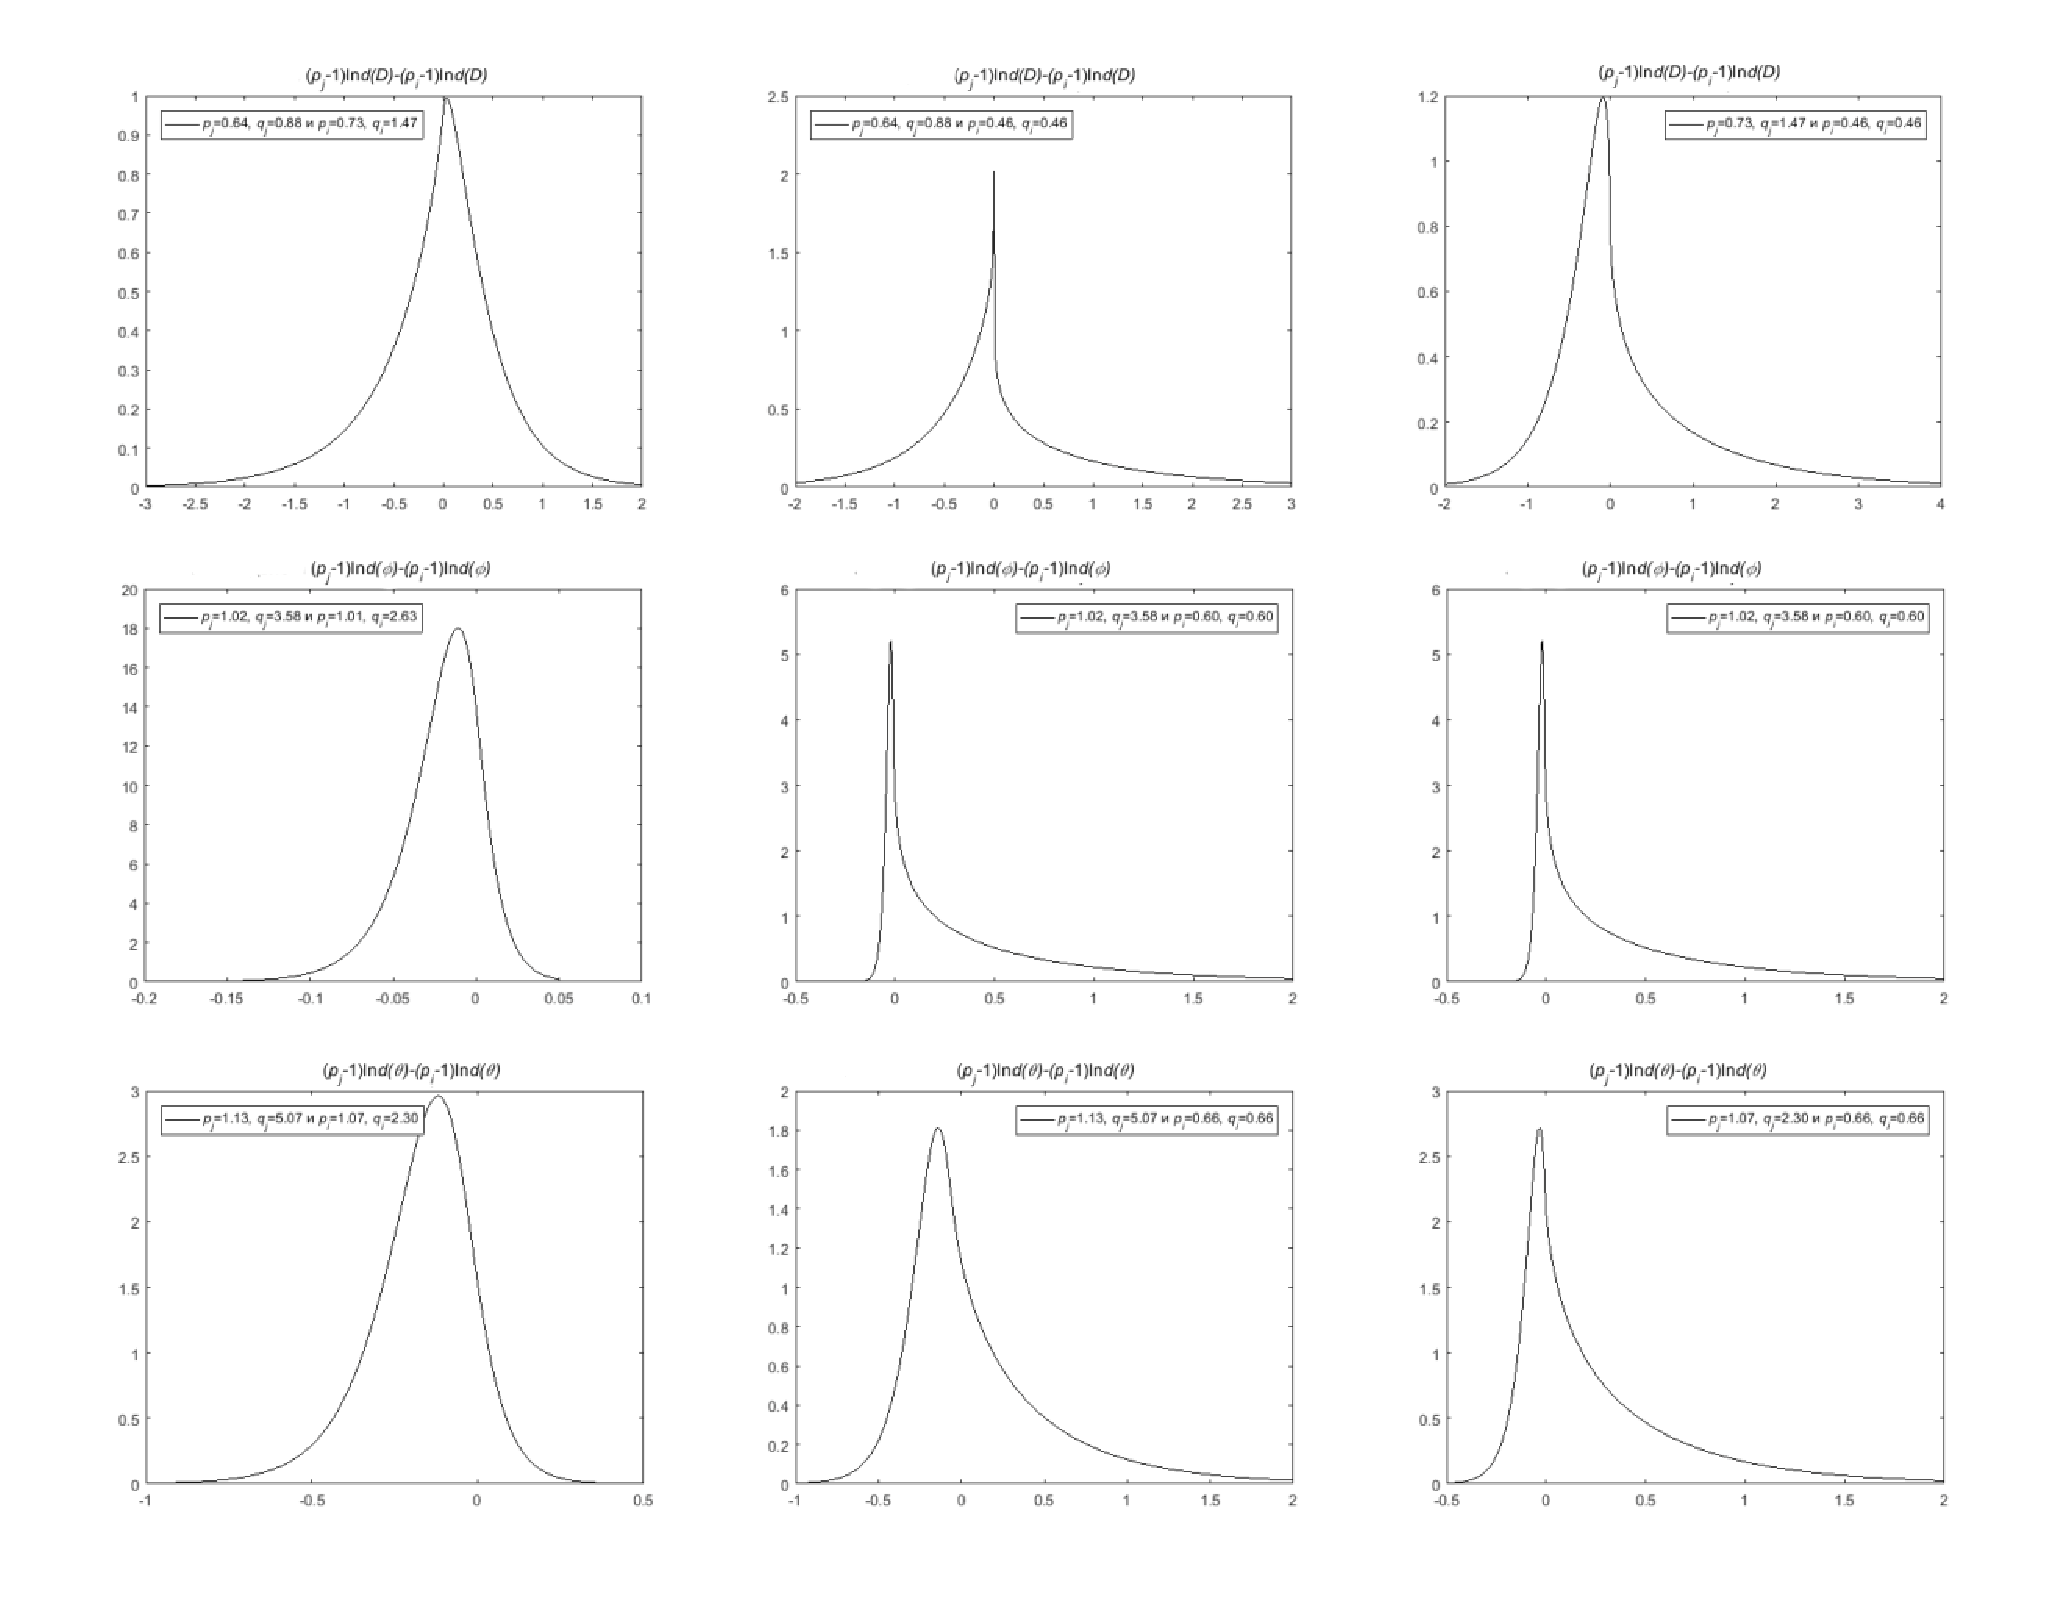
\includegraphics[width=1.0\textwidth]{pics/fig_2.pdf}
\captionstyle{normal}\caption{The laws of the distribution of statistics functions of fractal dimension.}\label{fig:fig_2}
\end{figure}

\begin{figure}[h]
\setcaptionmargin{5mm}
\onelinecaptionstrue
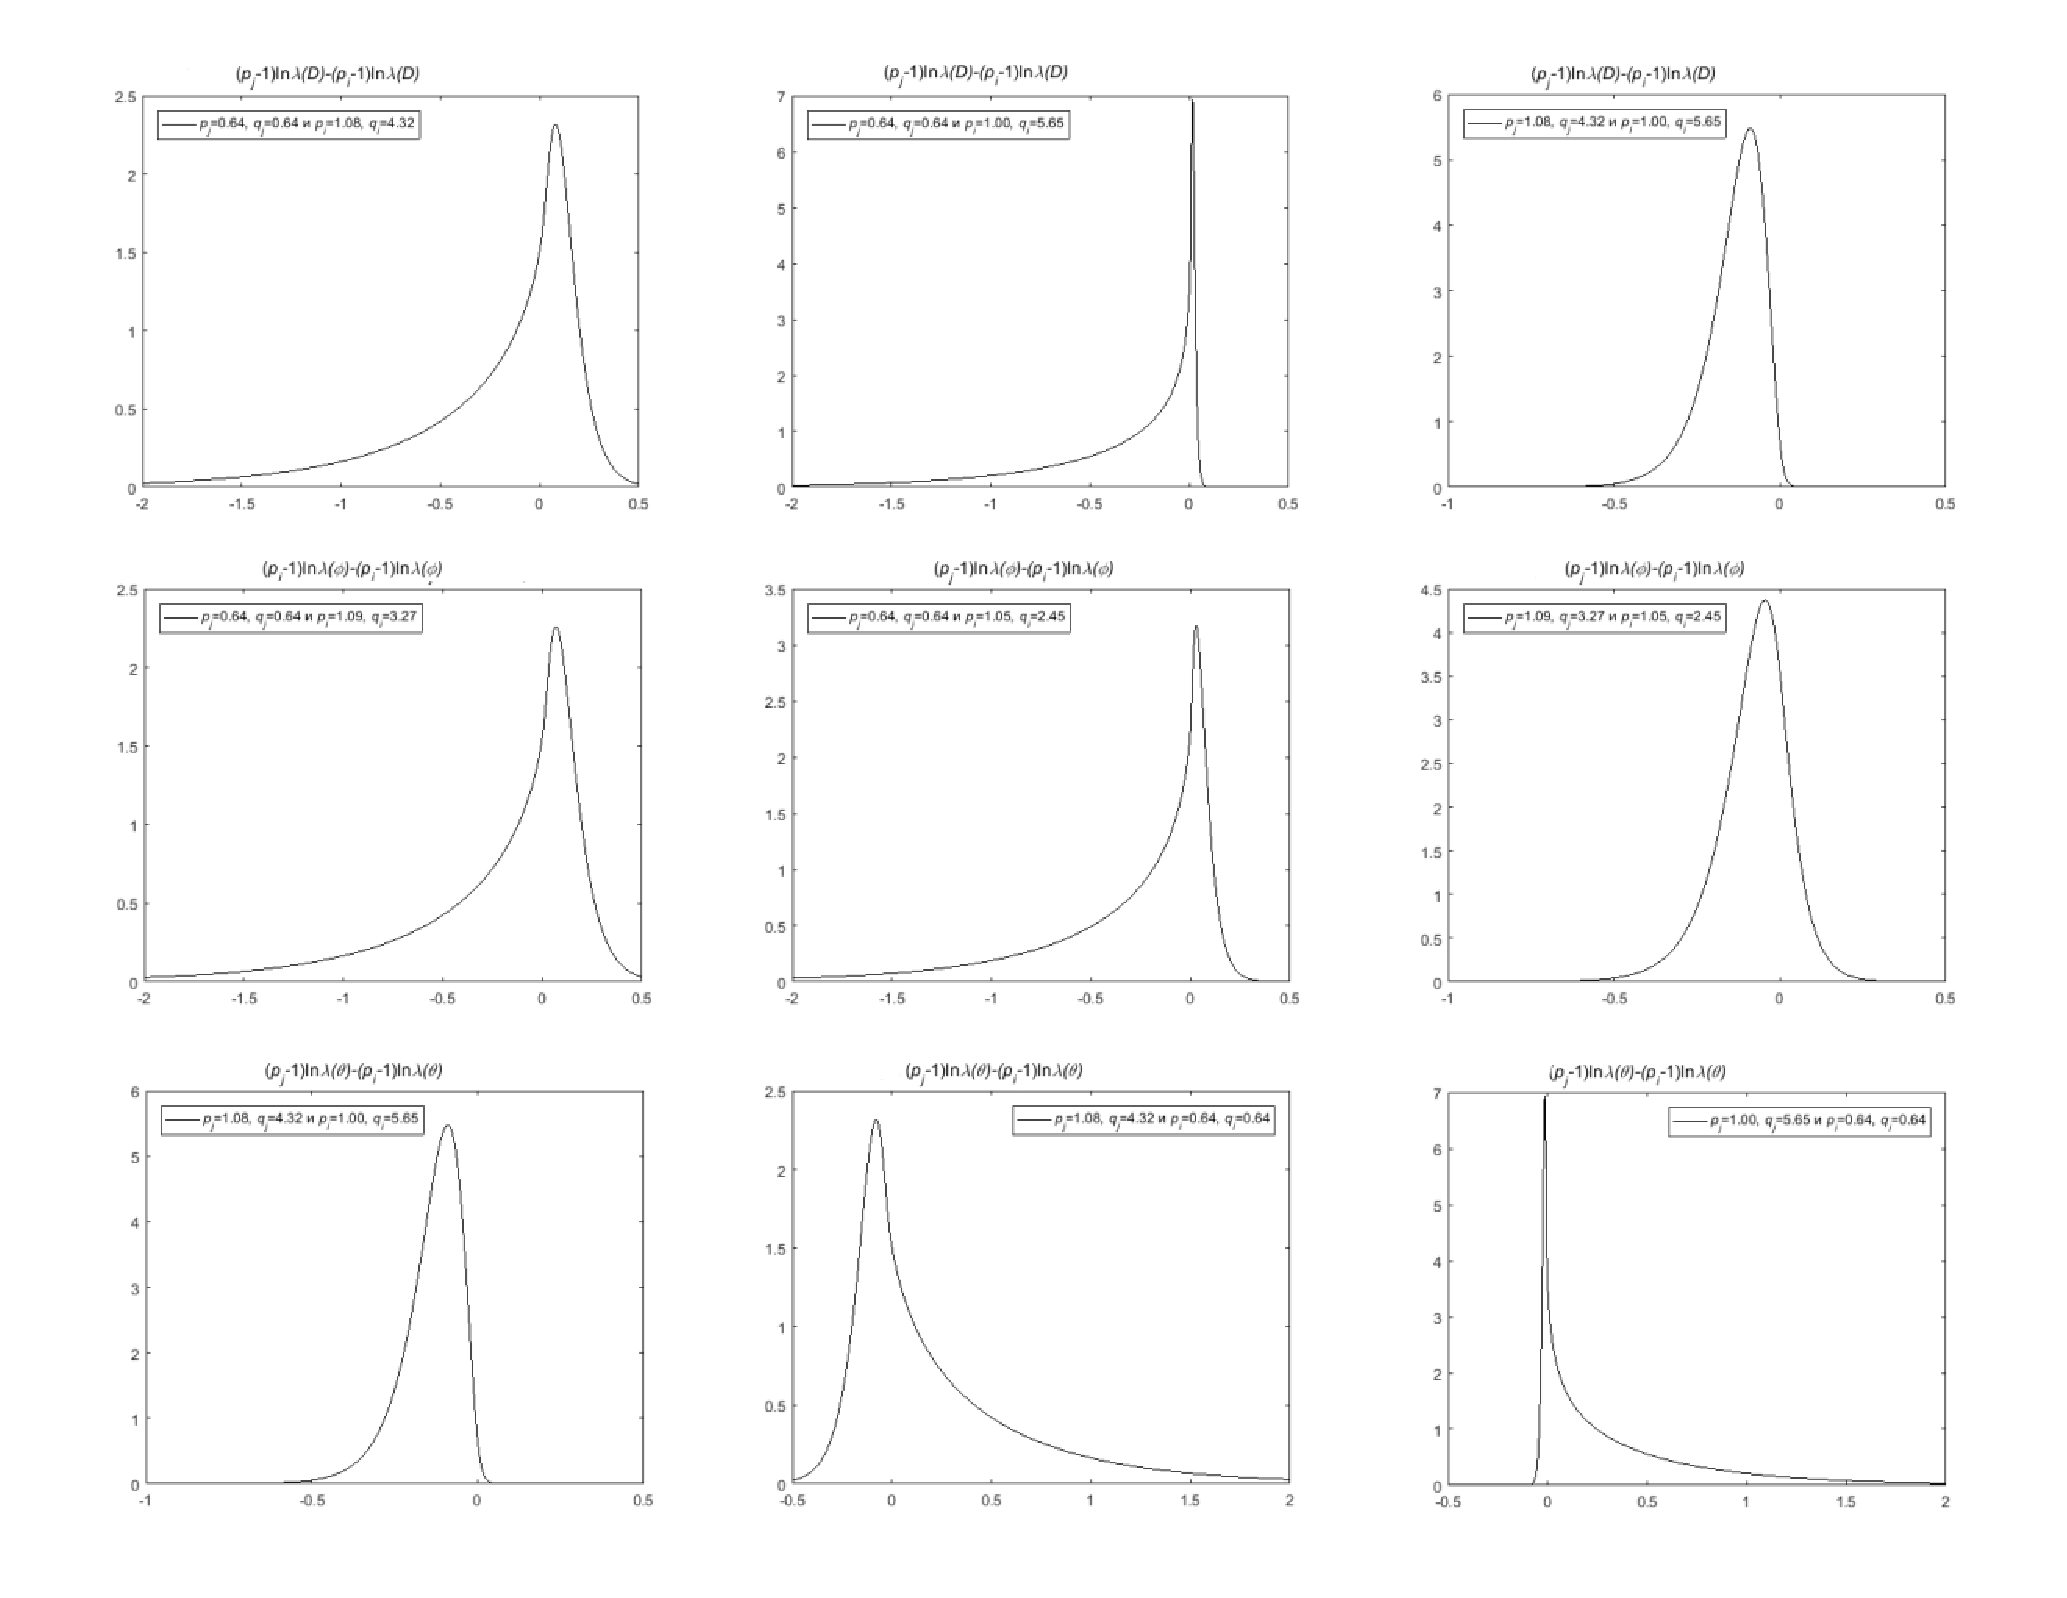
\includegraphics[width=1.0\textwidth]{pics/fig_3.pdf}
\captionstyle{normal}\caption{The laws of the distribution of statistics functions of maximum eigenvalue.}\label{fig:fig_3}
\end{figure}

\begin{figure}[h]
\setcaptionmargin{5mm}
\onelinecaptionstrue
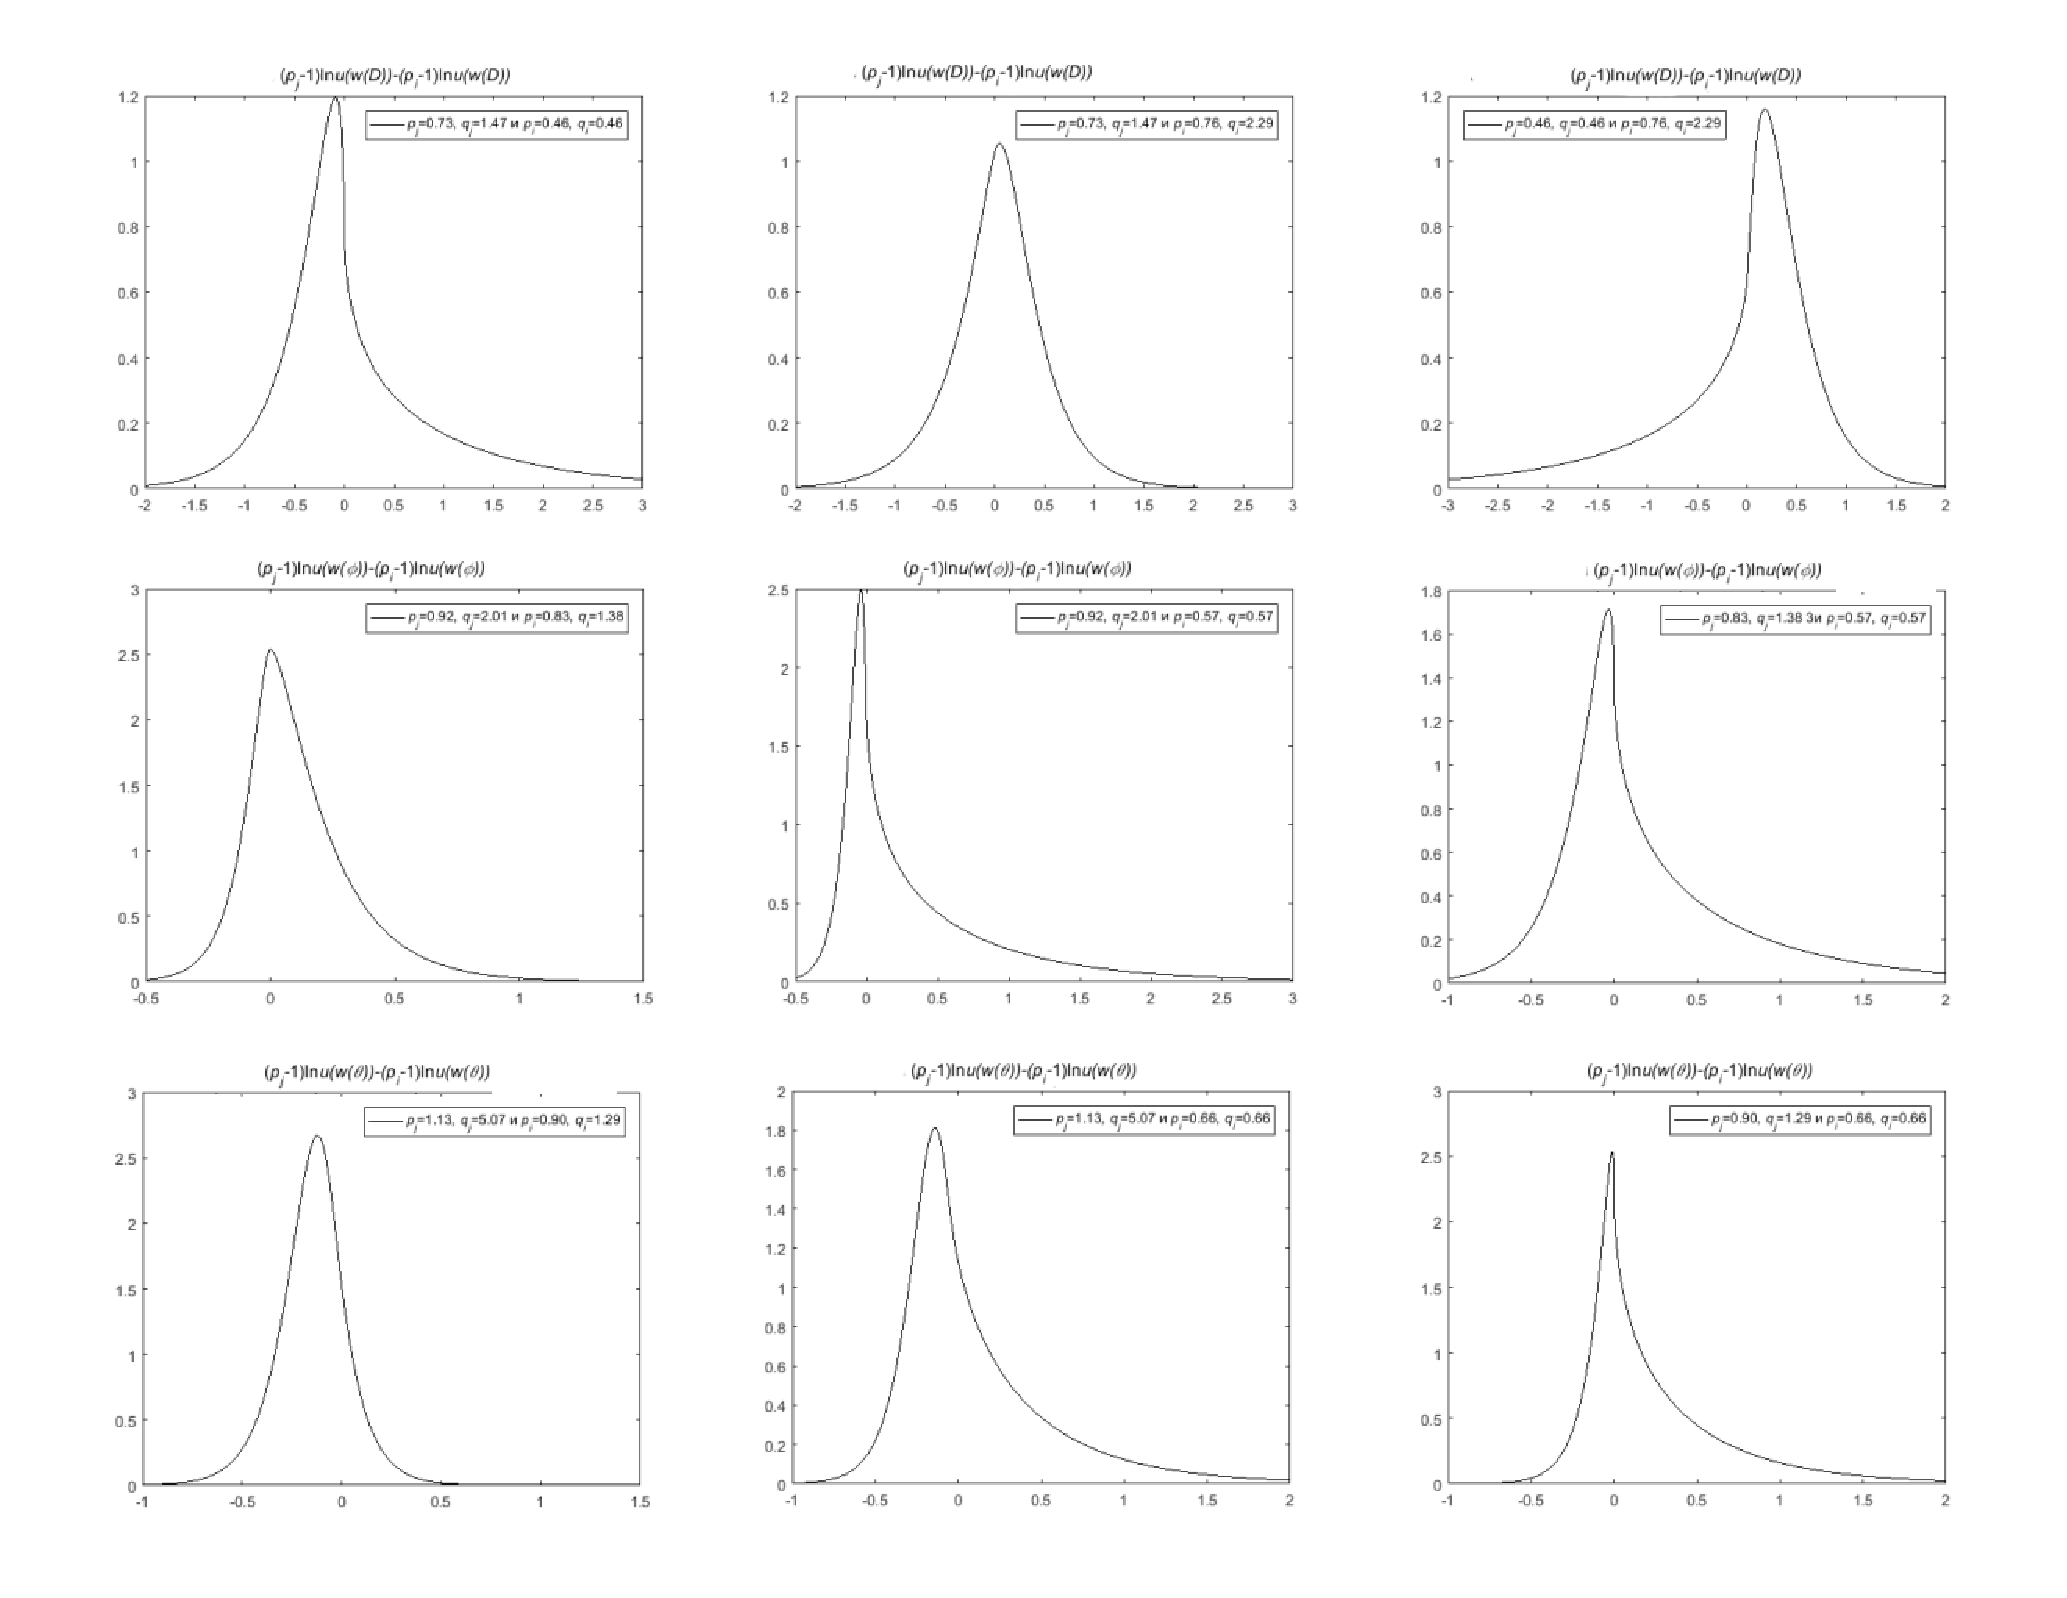
\includegraphics[width=1.0\textwidth]{pics/fig_4.pdf}
\captionstyle{normal}\caption{The laws of the distribution of the statistics functions of the energy of the wavelet spectrum.}\label{fig:fig_4}
\end{figure}


\section{Performance indicators of DO type identification algorithm}

performance TODO

\section{Conclusion}

It is established the invariance of the structure of the wavelet-fractal-correlation DO type identification algorithm to the peculiarities of the current phono-target environment controlled by OED.

The statistical stability of the initial sufficient statistics for the algorithm and the statistical stability of DO type identification algorithm itself are proved for various features of its flight path and sight.

The performance indicators of the wavelet-fractal-correlation type recognition algorithm are estimated for various real-world operating conditions of the OED as the primary sensor of the sets of measurements of the coordinates of the elevation angle, azimuth and range of the detected DO at each finite current time interval and the stable performance of the algorithm in both simple and complex phono-target conditions for the functioning of the OED, including during intensive maneuvering of DO.

Set forth above it represents the development of the theory of methods for assessing the stability of the functioning of algorithms in the conditions of statistical and tactical uncertainty about the current phono-target situation in the zone of control of OED.


\begin{thebibliography}{99}

\bibitem{bib_01}
\refitem{article}
A.~N.~Katulev, A.~A.~Khramichev, {\it ``A wavelet-fractal-correlation algorithm for recognizing the type of a dynamic object detected on a finite sequence of 2D phonon-image frames of an optoelectronic device"}, Optical Journal, T.~84, 1--10 (2017).

\bibitem{bib_02}
\refitem{book}
A.~A.~Potapov, Yu.~V.~Gulyaev, S.~A.~Nikitov, A.~A.~Pakhomov, V.~A.~German, {\it ``The newest methods of image processing"}, Moscow: Fizmatlit, 496 p. (2008).

\bibitem{bib_03}
\refitem{book}
V.~A.~Ponkin, E.~V.~Peteshchenkov, E.~M.~Afanasyeva, {\it ``Optical visibility of aircraft"}, Voronezh: "The Scientific Book", 553 p. (2015).

\bibitem{bib_04}
\refitem{book}
B.~A.~Alpatov, P.~V.~Babayan, O.~E.~Balashov, A.~I.~Stepashkin, {\it ``Methods of automatic detection and tracking of objects. Image processing and management"}, Moscow: Radio Engineering, 176 p. (2008).

\bibitem{bib_05}
\refitem{article}
Autometry, T.~50, No.~1--6 (2014); T.~51, No.~1--6 (2015); T.~52, No.~1--5 (2016).

\bibitem{bib_06}
\refitem{article}
Computeroptics, T.~37, 38, 39, 40 (2013--2016).

\bibitem{bib_07}
\refitem{book}
G.~I.~Ivchenko, Yu.~I.~Medvedev, {\it ``Math statistics"}, Moscow: VSh, 248 p. (1984).

\bibitem{bib_08}
\refitem{book}
{\it ``Directory of the officer of aerospace defense"}, Tver, 564 p. (2008).

\bibitem{bib_09}
\refitem{book}
D.~Cox, D.~Hinckley, {\it ``Theoretical statistics"}, Moscow: Mir, 560 p. (1978).

\bibitem{bib_10}
\refitem{article}
S.~Wilks, {\it ``Mathematical statistics"}, Moscow: Nauka, 632 p. (1967).

\bibitem{bib_11}
\refitem{book}
P.~Huber, {\it ``Robustness in statistics"}, Moscow: Mir, 304 p. (1984).

\bibitem{bib_12}
\refitem{book}
A.~K.~Mitropolsky, {\it ``The technique of statistical computations"}, Moscow: Nauka, 576 p. (1971).

\bibitem{bib_13}
\refitem{book}
G.~Kramer, {\it ``Mathematical methods of statistics"}, M.: The World, 648 p. (1975).

\bibitem{bib_14}
\refitem{book}
N.~V.~Smirnov, I.~V.~Dunin-Barkovsky, {\it ``A short course of mathematical statistics for technical applications"}, Moscow: FML, 436 p. (1959).

\bibitem{bib_15}
\refitem{book}
N.~A.~Livshits, V.~N.~Pugachev, {\it ``Probabilistic analysis of automatic control systems"}, Moscow: Sov. Radio, 896 p. (1963).

\bibitem{bib_16}
\refitem{book}
S.~A.~Aivazyan, I.~S.~Enyukov, L.~D.~Meshalkin, {\it ``Applied statistics, Т.~1, Fundamentals of modeling and primary data processing"},  Moscow: Finances and Statistics, 471 p. (1983).

\bibitem{bib_17}
\refitem{book}
A.~N.~Kolmogorov, S.~V.~Fomin, {\it ``Elements of the theory of functions and functional analysis"}, M.: Science, 406 p. (1968).

\bibitem{bib_18}
\refitem{book}
V.~S.~Korolyuk, N.~I.~Portenko, A.~V.~Skorokhod, A.~F.~Turbin, {\it ``A handbook on probability theory and mathematical statistics"}, Moscow: Nauka, 640 p. (1985).

\bibitem{bib_19}
\refitem{book}
Yu.~V.~Prokhorov, Yu.~A.~Rozanov, {\it ``Probability theory. Basic concepts. Limit theorems. Random processes"}, Moscow: Nauka, 406 p. (1967).

\bibitem{bib_20}
\refitem{book}
A.~E.~Basharinov, B.~S.~Fleishman, {\it ``Methods of statistical sequential analysis and their radio engineering applications"}, Moscow: Sov. Radio, 352 p. (1962).

\bibitem{bib_21}
\refitem{book}
S.~Z.~Kuzmin, {\it ``Fundamentals of the theory of digital processing of radar information"}, Moscow: Sov. Radio, 432 p. (1974).

\bibitem{bib_22}
\refitem{book}
V.~A.~Malyshev, I.~M.~Khmarov, O.~V.~Malyshev etc., {\it ``Recognition of surface objects and aircrafts by 2D and 3D optoelectronic systems"}, Moscow: FGUP NTC Informatika, 158 p. (2013).

\end{thebibliography}

\end{document}
